%%%%%%%%%%%%%%%%%%%%%%%%%%%%%%%%%%%%%%%%%
% Masters/Doctoral Thesis 
% LaTeX Template
% Version 2.3 (25/3/16)
%
% This template has been downloaded from:
% http://www.LaTeXTemplates.com
%
% Version 2.x major modifications by:
% Vel (vel@latextemplates.com)
%
% This template is based on a template by:
% Steve Gunn (http://users.ecs.soton.ac.uk/srg/softwaretools/document/templates/)
% Sunil Patel (http://www.sunilpatel.co.uk/thesis-template/)
%
% Template license:
% CC BY-NC-SA 3.0 (http://creativecommons.org/licenses/by-nc-sa/3.0/)
%
%%%%%%%%%%%%%%%%%%%%%%%%%%%%%%%%%%%%%%%%%

%----------------------------------------------------------------------------------------
%	PACKAGES AND OTHER DOCUMENT CONFIGURATIONS
%----------------------------------------------------------------------------------------

\documentclass[
11pt, % The default document font size, options: 10pt, 11pt, 12pt
%oneside, % Two side (alternating margins) for binding by default, uncomment to switch to one side
%chapterinoneline,% Have the chapter title next to the number in one single line
%english, % ngerman for German
spanish,
singlespacing, % Single line spacing, alternatives: onehalfspacing or doublespacing
%draft, % Uncomment to enable draft mode (no pictures, no links, overfull hboxes indicated)
%nolistspacing, % If the document is onehalfspacing or doublespacing, uncomment this to set spacing in lists to single
%liststotoc, % Uncomment to add the list of figures/tables/etc to the table of contents
%toctotoc, % Uncomment to add the main table of contents to the table of contents
parskip, % Uncomment to add space between paragraphs
%nohyperref, % Uncomment to not load the hyperref package
headsepline, % Uncomment to get a line under the header
]{MastersDoctoralThesis} % The class file specifying the document structure



\usepackage[utf8]{inputenc} % Required for inputting international characters
\usepackage[T1]{fontenc} % Output font encoding for international characters

\usepackage{palatino} % Use the Palatino font by default
%,style=authoryear
\usepackage[backend=bibtex,natbib=true,style=authoryear]{biblatex} % Use the bibtex backend with the authoryear citation style (which resembles APA)

\addbibresource{references.bib} % The filename of the bibliography

\usepackage[autostyle=true]{csquotes} % Required to generate language-dependent quotes in the bibliography

\usepackage{caption}
\usepackage{subcaption}

%------------------------
\usepackage{listings}

%\usepackage[hyphens]{url}
%\usepackage[hidelinks]{hyperref}
%\hypersetup{breaklinks=true}
\urlstyle{same}
%\usepackage{cite}

%--------------------------

\usepackage{color}

\hyphenation{Dunkel successful}

%
%----------------------------------------------------------------------------------------
%	MARGIN SETTINGS
%----------------------------------------------------------------------------------------

\geometry{
	paper=a4paper, % Change to letterpaper for US letter
	inner=2cm, % Inner margin
	outer=3.3cm, % Outer margin
	bindingoffset=2cm, % Binding offset
	top=1.5cm, % Top margin
	bottom=1.5cm, % Bottom margin
	%showframe,% show how the type block is set on the page
}

%----------------------------------------------------------------------------------------
%	INFORMACIÓN DE LA MEMORIA
%----------------------------------------------------------------------------------------

\thesistitle{Sistema de control para estación autónoma de monitoreo de ruido ambiente submarino} % El títulos de la memoria, se usa en la carátula y se puede usar el cualquier lugar del documento con el comando \ttitle
\supervisor{Dr. Ing. Ariel Lutenberg} % El nombre del director, se usa en la carátula y se puede usar el cualquier lugar del documento con el comando \supname
\degree{Magíster en Sistemas Embebidos } % Nombre del grado, se usa en la carátula y se puede usar el cualquier lugar del documento con el comando \degreename
\author{Patricio Bos} % Tu nombre, se usa en la carátula y se puede usar el cualquier lugar del documento con el comando \authorname
\juradoUNO{Dr. Ing Pablo Gómez (FIUBA)} % Nombre y pertenencia del un jurado se usa en la carátula y se puede usar el cualquier lugar del documento con el comando \jur1name
\juradoDOS{Ing. Juan Manuel Cruz (FIUBA, UTN-FRBA)} % Nombre y pertenencia del un jurado se usa en la carátula y se puede usar el cualquier lugar del documento con el comando \jur2name
\juradoTRES{Mg. Lic. Igor Prario (FIUBA)} % Nombre y pertenencia del un jurado se usa en la carátula y se puede usar el cualquier lugar del documento con el comando \jur3name
\fechaINICIO{enero de 2017}
\fechaFINAL{diciembre de 2018}

\subject{Memoria del Trabajo Final de la Maestría en Sistemas Embebidos de la UBA} % Your subject area, this is not currently used anywhere in the template, print it elsewhere with \subjectname
\keywords{MSE, Sistemas Embebidos, CIAA} % Keywords for your thesis, this is not currently used anywhere in the template, print it elsewhere with \keywordnames
\university{Universidad de Buenos Aires} % Your university's name and URL, this is used in the title page and abstract, print it elsewhere with \univname
\faculty{{Facultad de Ingeniería}} % Your faculty's name and URL, this is used in the title page and abstract, print it elsewhere with \facname
\department{Departamento de Electrónica} % Your department's name and URL, this is used in the title page and abstract, print it elsewhere with \deptname
\group{{Laboratorio de Sistemas Embebidos}} % Your research group's name and URL, this is used in the title page, print it elsewhere with \groupname


\hypersetup{pdftitle=\ttitle} % Set the PDF's title to your title
\hypersetup{pdfauthor=\authorname} % Set the PDF's author to your name
\hypersetup{pdfkeywords=\keywordnames} % Set the PDF's keywords to your keywords


\newcaptionname{spanish}{\acknowledgementname}{Agradecimientos}
\newcaptionname{spanish}{\authorshipname}{Declaración de Autoría}
\newcaptionname{spanish}{\abbrevname}{Glosario}
\newcaptionname{spanish}{\byname}{por}

\renewcommand{\lstlistingname}{Algoritmo}% Listing -> Algorithm
\renewcommand{\lstlistlistingname}{Índice de \lstlistingname s}% List of Listings -> List of Algorithms

\renewcommand{\listtablename}{Índice de Tablas}
\renewcommand{\tablename}{Tabla} 

\renewcommand{\labelenumi}{\arabic{enumi}.} 
\renewcommand{\labelenumii}{\arabic{enumi}.\arabic{enumii}}


\addtolength{\footnotesep}{2mm} % Espacio adicional en los footnotes

\begin{document}

\frontmatter % Use roman page numbering style (i, ii, iii, iv...) for the pre-content pages

\pagestyle{plain} % Default to the plain heading style until the thesis style is called for the body content

%----------------------------------------------------------------------------------------
%	CARÁTULA
%----------------------------------------------------------------------------------------

\begin{titlepage}
\begin{center}

{\scshape\LARGE UNIVERSIDAD DE BUENOS AIRES\par}\vspace{0.1cm} % University name
{\scshape\LARGE FACULTAD DE INGENIERÍA\par}\vspace{0.1cm} % Faculty name
{\scshape\LARGE Maestría en Sistemas Embebidos\par}\vspace{1cm} % Thesis type


\includegraphics[width=.3\textwidth]{./Figures/logoFIUBA.png}
\vspace{1cm}

\textsc{\Large Memoria del Trabajo Final}\\[0.5cm] % Thesis type

{\huge \bfseries \ttitle\par}\vspace{0.4cm} % Thesis title

\vspace{1cm}
\LARGE\textbf{Autor:\\
\authorname}\\ % Author name

\vspace{1cm}

\large
\vspace{10px}
{Director:} \\
{\supname} % Supervisor name
 
\vspace{1cm}
Jurados:\\
\jurunoname\\
\jurdosname\\
\jurtresname
 
\vfill
\textit{Este trabajo fue realizado en las Ciudad Autónoma de Buenos Aires, entre \fechaINICIOname \hspace{1px} y \fechaFINALname.}
\end{center}
\end{titlepage}


%----------------------------------------------------------------------------------------
%	RESUMEN - ABSTRACT 
%----------------------------------------------------------------------------------------

\begin{abstract}
\addchaptertocentry{\abstractname} % Add the abstract to the table of contents
%
%The Thesis Abstract is written here (and usually kept to just this page). The page is kept centered vertically so can expand into the blank space above the title too\ldots
\centering

La presente memoria describe el diseño e implementación de un sistema embebido para el control de una estación de monitoreo de ruido ambiente submarino. El sistema integra y almacena información de distintos sensores y provee una interfaz para la configuración de la estación. A su vez, permite operar con distintos perfiles de consumo de energía. El conocimiento del nivel de ruido submarino es importante para distintas disciplinas dentro de la oceanografía acústica, estudios de impacto ambiental y diversas aplicaciones que utilicen sistemas SONAR dentro del ámbito científico, civil y militar, entre otras.

Este documento incluye la información de trazabilidad de requerimientos.  Se detalla la arquitectura multicore utilizada, junto con los mecanismos de comunicación y sincronización implementados. Asimismo, se describen las técnicas de ingeniería de software aplicadas y el modelo de ramas adoptado para el desarrollo con control de versiones. Finalmente, se incluye la documentación de testing y los resultados obtenidos.					
\end{abstract}

%----------------------------------------------------------------------------------------
%	CONTENIDO DE LA MEMORIA  - AGRADECIMIENTOS
%----------------------------------------------------------------------------------------

\begin{acknowledgements}
%\addchaptertocentry{\acknowledgementname} % Descomentando esta línea se puede agregar los agradecimientos al índice
\vspace{1.5cm}

Agradecimientos personales. \textbf{[OPCIONAL]} 

No olvidarse de agradecer al tutor.

No vale poner anti-agradecimientos (este trabajo fue posible a pesar de...)

\end{acknowledgements}

%----------------------------------------------------------------------------------------
%	LISTA DE CONTENIDOS/FIGURAS/TABLAS
%----------------------------------------------------------------------------------------
%\renewcommand{\listtablename}{Índice de Tablas}

\tableofcontents % Prints the main table of contents

\listoffigures % Prints the list of figures

\listoftables % Prints the list of tables


%----------------------------------------------------------------------------------------
%	CONTENIDO DE LA MEMORIA  - DEDICATORIA
%----------------------------------------------------------------------------------------

%\dedicatory{\textbf{Dedicado con cariño a Carla, Dante y le bebé sin los cuales este trabajo se hubiera terminado 2 años antes. }}  

%----------------------------------------------------------------------------------------
%	CONTENIDO DE LA MEMORIA  - CAPÍTULOS
%----------------------------------------------------------------------------------------

\mainmatter % Begin numeric (1,2,3...) page numbering

\pagestyle{thesis} % Return the page headers back to the "thesis" style

\renewcommand{\tablename}{Tabla} 

% Incluir los capítulos como archivos separados desde la carpeta Chapters
% Descomentar las líneas a medida que se escriben los capítulos

% Chapter 1

\chapter{Introducción General} % Main chapter title

\label{Chapter1} % For referencing the chapter elsewhere, use \ref{Chapter1} 
\label{IntroGeneral}

%----------------------------------------------------------------------------------------

% Define some commands to keep the formatting separated from the content 
\newcommand{\keyword}[1]{\textbf{#1}}
\newcommand{\tabhead}[1]{\textbf{#1}}
\newcommand{\code}[1]{\texttt{#1}}
\newcommand{\file}[1]{\texttt{\bfseries#1}}
\newcommand{\option}[1]{\texttt{\itshape#1}}
\newcommand{\grados}{$^{\circ}$}

%----------------------------------------------------------------------------------------

En este capítulo se introduce brevemente el campo de la acústica submarina y la importancia del parámetro SONAR Ruido Ambiente Submarino como motivación para la realización de este trabajo.  Se presentan los objetivos y el alcance del proyecto.
%----------------------------------------------------------------------------------------
\section{Descripción técnica-conceptual del proyecto}

%Contexto que da origen al proyecto de investigación.
%Introducción conceptos de acústica submarina.
%Qué es el ruido submarino.
%Cómo se mide / intro hidrófono.

La acústica submarina estudia la propagación del sonido en el agua y la interacción de las ondas mecánicas que constituyen el sonido con el agua, los elementos dispersores presentes y las interfaces aire-agua y agua-lecho marino.  Debido a que sufre menor atenuación que otras formas de radiación, el sonido es ampliamente empleado  por el hombre en su exploración de los océanos.  Las frecuencias típicas utilizadas se encuentran en el rango comprendido entre $\sim$10 Hz y 1 MHz, dependiendo de la aplicación.  

Los sistemas que utilizan la propagación del sonido bajo el agua con diversos fines se conocen como sistemas SONAR (\textit{\textbf{SO}und \textbf{N}avigation \textbf{A}nd \textbf{R}anging}).

La propagación del sonido en el agua depende de diversos factores.  La dirección de propagación está determinada principalmente por el gradiente vertical de velocidades del sonido, que a su vez depende fundamentalmente de la temperatura y la salinidad del agua.  El perfil de velocidades del sonido puede causar zonas de baja intensidad del sonido, llamadas ``zonas de sombra'', y regiones de alta intensidad llamadas ``cáusticas''. Estas zonas pueden hallarse con el método de trazado de rayos \citep{tappert1977parabolic}.

El sonido en el agua puede propagarse a grandes distancias, en el orden de miles de kilómetros, debido a la presencia de un canal especial que actúa como guía de onda para el sonido, conocido como SOFAR (\textbf{SO}und \textbf{F}ixing \textbf{A}nd \textbf{R}anging) que se produce, bajo ciertas condiciones, a la profundidad donde el gradiente de velocidades del sonido alcanza un mínimo \citep{medwin1997fundamentals}. 

Los distintos fenómenos que afectan al sonido submarino pueden ser conveniente y lógicamente agrupados en un pequeño número de parámetros conocidos como parámetros SONAR que se pueden relacionar entre sí mediante las ecuaciones SONAR \citep{urick1975principles}.  Estas ecuaciones exhiben las relaciones de trabajo que agrupan los efectos del medio de propagación, el blanco y el equipamiento utilizado y constituyen las herramientas básicas para los profesionales que trabajen en aplicaciones de acústica submarina. 

En el campo de la acústica submarina resulta muy relevante el conocimiento del parámetro SONAR Nivel de Ruido en el mar (NL: \textit{Noise Level}), que incluye el Ruido Ambiente propiamente dicho (NLa) y el Ruido Propio (NLp) asociado al sistema de medición. En el caso de escucha pasiva (estudios de impacto ambiental sobre mamíferos marinos a bajas frecuencias o detección subacuática efectuada desde vehículos submarinos), el NL está dominado por el NLa.

Conceptualmente, el Nivel de Ruido en el mar está asociado al ruido de ``fondo'' (\textit{background}) remanente en ausencia de toda otra fuente identificable. Es el nivel de energía acústica mínimo que debe tener una señal para ser detectada.

Cabe destacar que el ruido subacuático puede clasificarse esencialmente en tres tipos:

\begin{itemize}
	\item Ambiente: comúnmente denominado ruido de fondo, se mide omnidireccionalmente y es originado principalmente por ruido en la superficie marina (debido al viento, oleaje o lluvia), ruido de origen biológico (producido por peces, mamíferos e invertebrados), ruido sísmico o geoacústico natural, ruido de tráfico marítimo (originado por tráfico marítimo distante).
	\item Ruido Radiado: originado por una fuente específica tal como un buque en particular, plataformas de explotación de petróleo o gas, instalaciones de exploración y perforación, instalaciones de generación eléctrica, etc.
	\item Ruido Propio: generado por el propio sistema de electrónico de medición de ruido y por la plataforma donde se encuentre instalado.
\end{itemize} 

El objetivo de este proyecto consiste en diseñar e implementar un sistema embebido para controlar una estación autónoma para la medición in-situ del ruido ambiente submarino para ser instalada en regiones de interés en el mar argentino y con la capacidad de transmitir datos a una estación receptora en tierra. Este desarrollo permitirá disponer de series temporales de ruido ambiente submarino durante períodos lo suficientemente largos como para analizar los resultados mediante modelos teóricos y/o empíricos que contribuyan a incrementar el conocimiento de dicho parámetro, especialmente a nivel local.

Se presenta un diagrama en bloques del sistema en la figura \ref{fig:diagramaBloques} donde se pueden observar los distintos módulos que componen el sistema.  En color verde los componentes asociados a la gestión de energía; en celeste los componentes asociados al almacenamiento de datos; en amarillo los componentes asociados a la gestión de las comunicaciones; en color azul los bloques del subsistema de adquisición de datos y finalmente, en color naranja se destaca el módulo central de procesamiento.

\begin{figure}[ht]
  \centering
	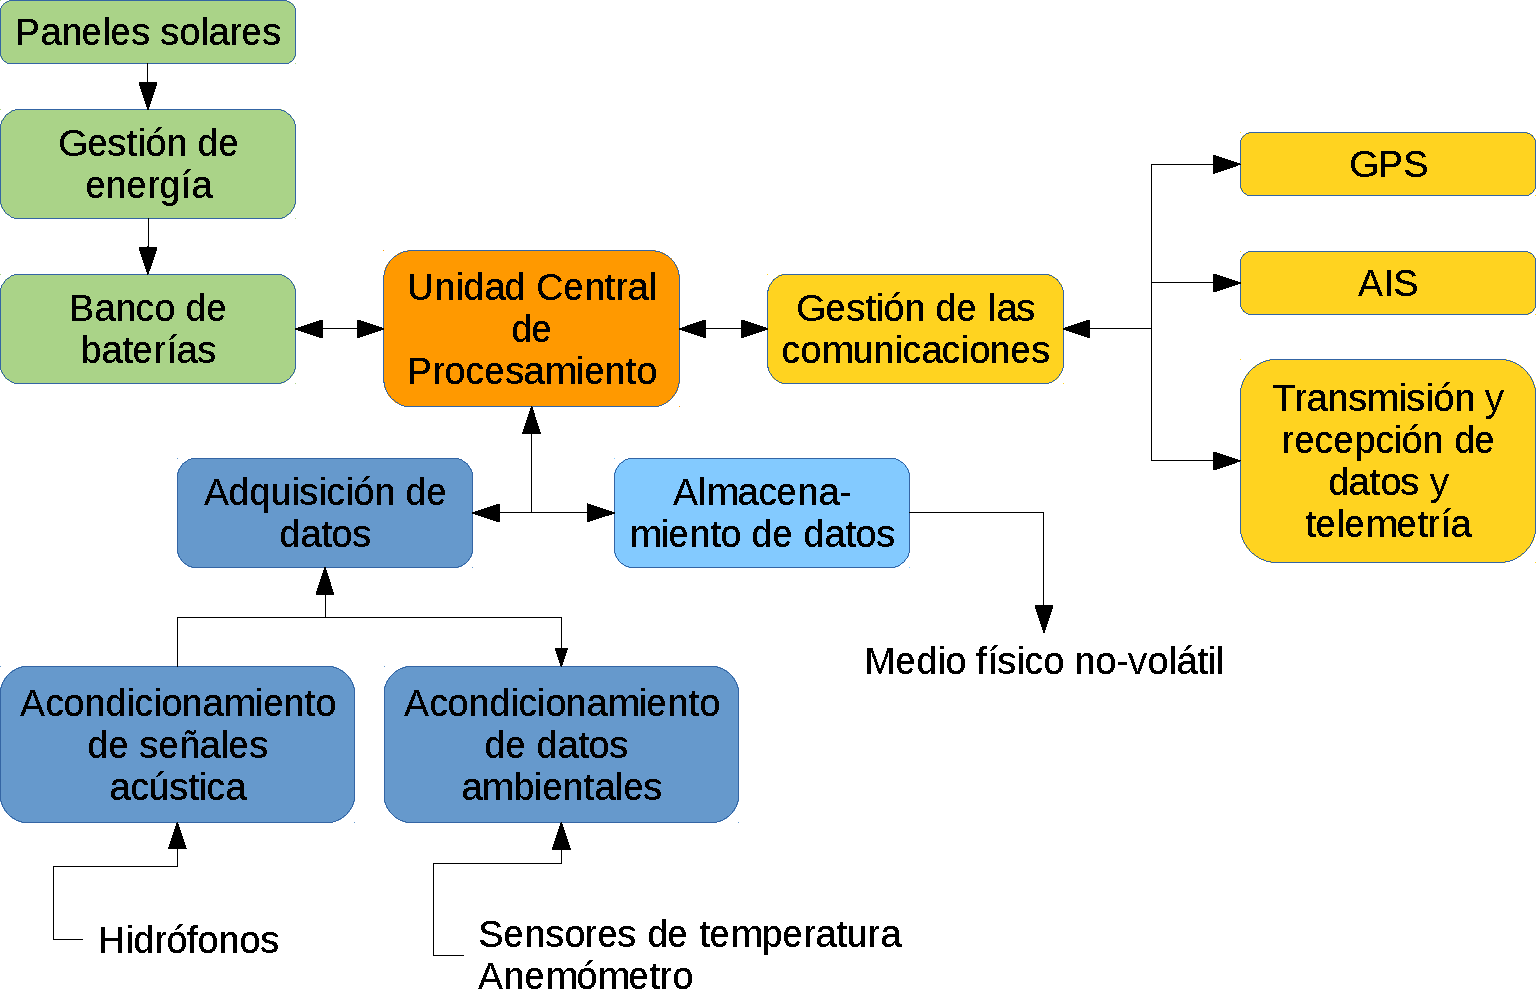
\includegraphics[width=\textwidth]{./Figures/Diagrama_en_Bloques.pdf}
	\caption[Diagrama en bloques general del sistema.]{Diagrama en bloques general. Se diferencian por color los sub-módulos funcionales: energía; unidad central de procesamiento; comunicaciones; adquisición y almacenamiento.}
	\label{fig:diagramaBloques}
\end{figure}

Para alcanzar el objetivo general se dispone de un paquete tecnológico compuesto principalmente por un equipo de trabajo multidisciplinario con conocimientos teóricos de los fenómenos físicos subyacentes a la propagación del sonido en el medio submarino, acceso a bibliografía especializada en acústica submarina y  conocimientos de ingeniería en el campo de los sistemas embebidos.

%Se presenta un diagrama en bloques del sistema en la figura \ref{fig:diagramaBloques} donde se han agrupado por color los distintos sub-módulos que conforman una misma área funcional.

%\begin{figure}
%	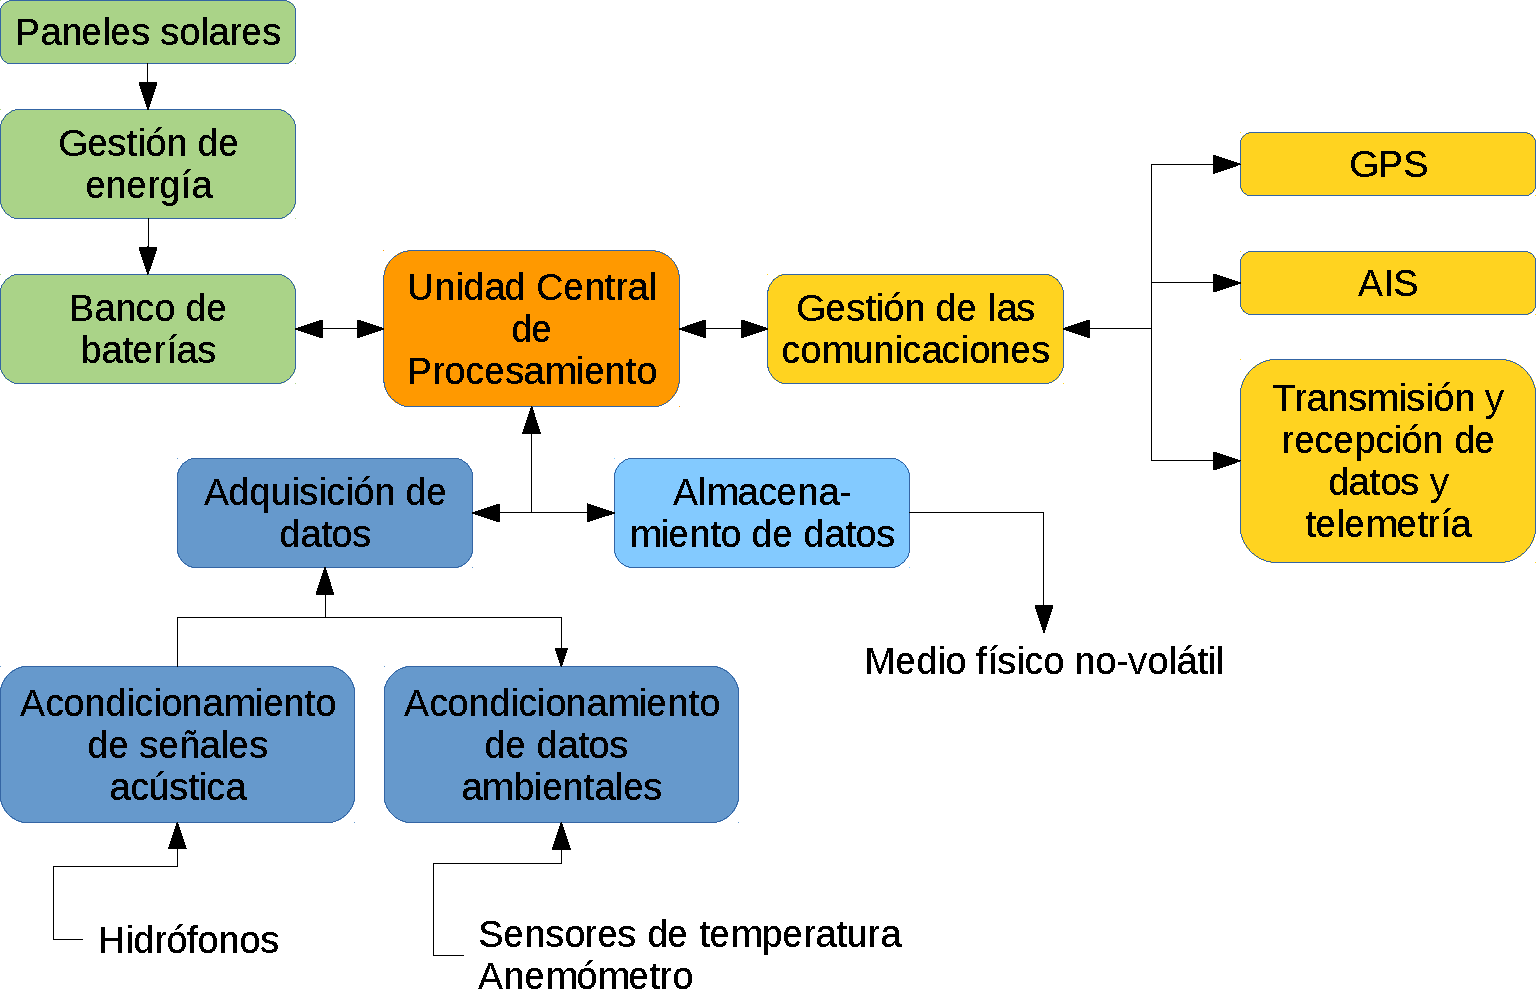
\includegraphics[width=\textwidth]{./Figures/Diagrama_en_Bloques.pdf}
%	\caption{Diagrama en bloques del sistema. Se diferencian por color los distintos sub-módulos funcionales.}
%	\label{fig:diagramaBloques}
%\end{figure}


%----------------------------------------------------------------------------------------

\section{Motivación}

%Para qué sirve medir el ruido submarino.

El conocimiento de valores de NL es fundamental en aplicaciones tales como oceanografía acústica, predicción SONAR, exploración geofísica, comunicación subacuática e ingeniería offshore, entre otras.

Por otra parte, existen muy pocas normas a nivel internacional para la estandarización de la medición in-situ del ruido ambiente subacuático. Si bien en acústica aérea sí existen estándares nacionales e internacionales muy aceptados, éstos no pueden extrapolarse fácilmente a la acústica subacuática dadas las diferentes características físicas del fluido en el cual se propaga el sonido, respectivamente.

Actualmente, en el ámbito de la comunidad científica internacional existe una creciente necesidad de medición y monitoreo del ruido subacuático. El interés está parcialmente motivado por un marco regulatorio internacional en lo concerniente al impacto ambiental del ruido subacuático de origen antrópico y principalmente para la evaluación de los efectos sobre la vida marina.


%----------------------------------------------------------------------------------------

\section{Objetivos y alcance}

%Objetivo del proyecto, recorte en el alcance

En particular, para el trabajo final de la Maestría en Sistemas Embebidos, se realizará una primera iteración sobre el ciclo de diseño centrada en la programación del sistema embebido que constituye la unidad central de procesamiento de la boya.  Se propone desarrollar sobre la plataforma CIAA-NXP, un firmware multicore de control que utilice ambos procesadores del microcontrolador LPC4337 y sea capaz de cumplir las siguientes funciones:

\begin{itemize}
	\item Adquirir datos ambientales de temperatura y velocidad de viento.
	\item Controlar el sistema mediante una interfaz serie.
	\item Almacenar los datos en una memoria no volátil.
\end{itemize}

En la primera iteración, se contempla la posibilidad de simular algún elemento del sistema según sea necesario para avanzar rápidamente en el diseño del firmware de control y las funciones mencionadas. 

A los fines prácticos de cumplir los requerimientos de tiempo del trabajo final de maestría, quedarán excluídos del diseño:

\begin{itemize}
	\item La transmisión de datos en tiempo real a una estación receptora en tierra.
	\item Consideraciones mecánicas del proyecto.
	\item La gestión de energía.
	\item La gestión y control del señalamiento reglamentario marítimo.
	\item La adquisición de señales acústicas.
\end{itemize}

Según un estudio preliminar, para el registro de señales acústicas resulta necesario una placa de adquisición A/D con características muy específicas en cuanto a frecuencia de muestreo, bits de resolución y figura de ruido, del tipo NI USB-6356 \cite{ni6356} o equivalente.  Este tipo de placas poseen \textit{drivers} propietarios cerrados que, en principio, no fue posible utilizar con la CIAA-NXP.   Por este motivo, la adquisición de señales acústicas también queda excluida del alcance en esta primera iteración.

Se muestra en la figura \ref{fig:diagramaBloquesReducido} un diagrama en bloques reducido con los componentes del sistema incluídos en la presente memoria.

\begin{figure}[ht]
  \centering
	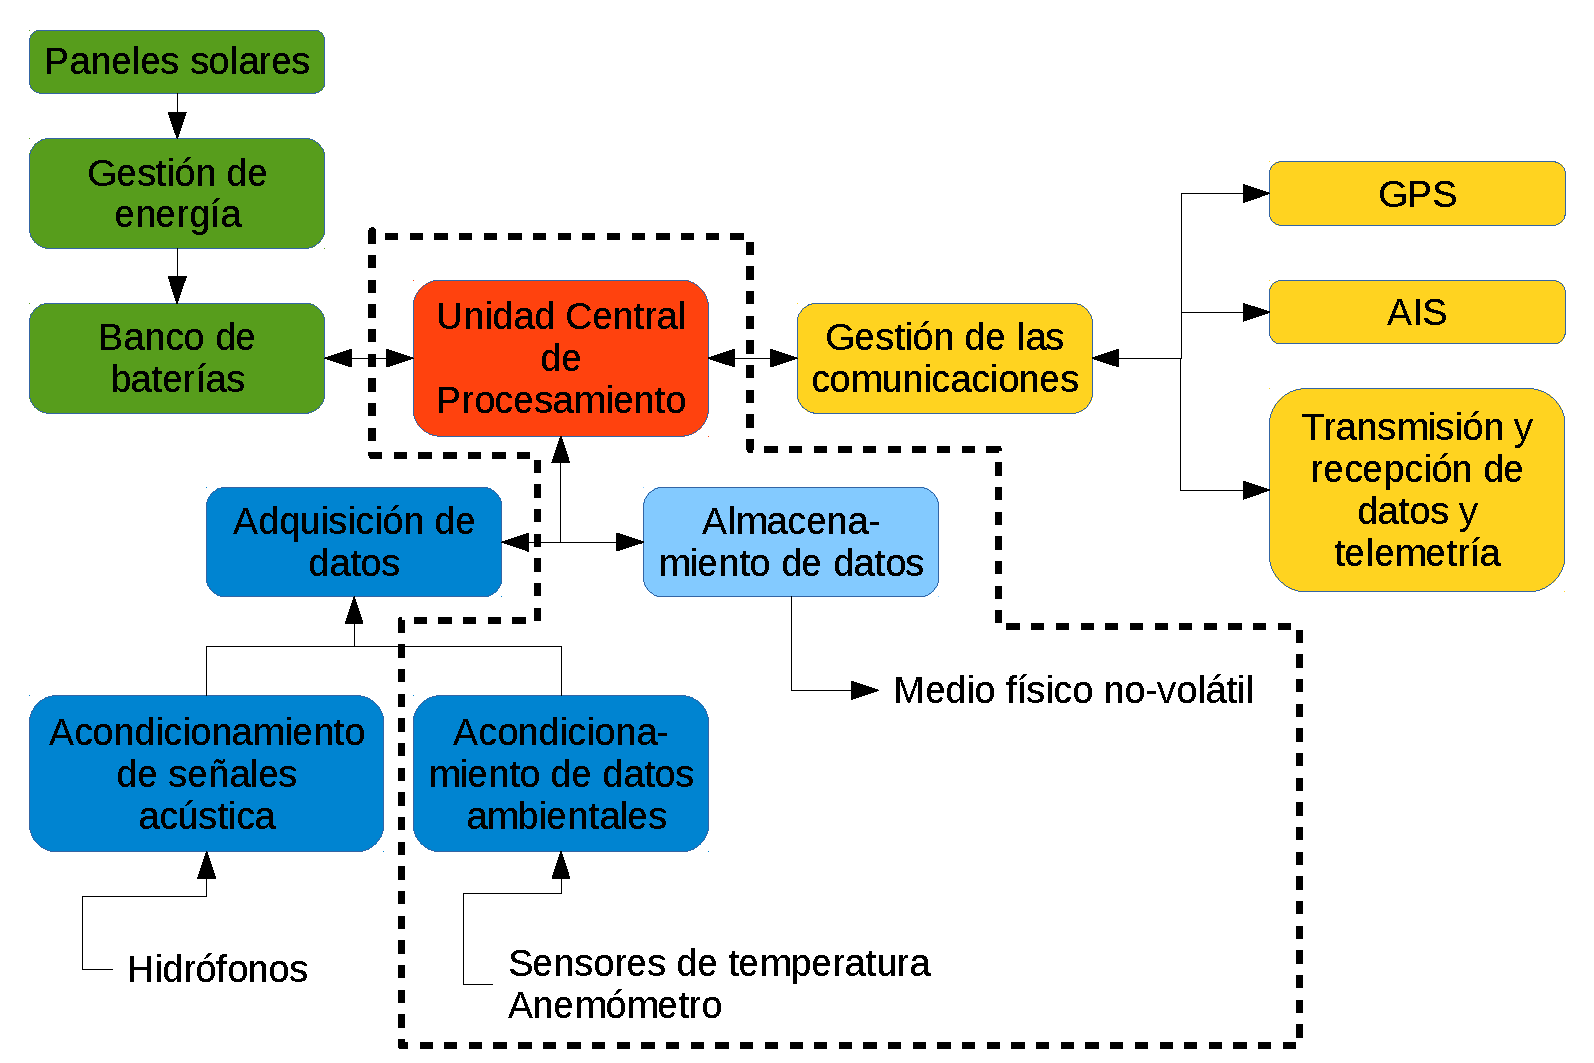
\includegraphics[width=.75\textwidth]{./Figures/Diagrama_en_Bloques_reducido.pdf}
	\caption[Diagrama en bloques implementado]{Diagrama en bloques del sistema implementado. Se diferencian por color los distintos sub-módulos funcionales incluidos en el alcance del proyecto.}
	\label{fig:diagramaBloquesReducido}
\end{figure}

%----------------------------------------------------------------------------------------





\chapter{Introducción Específica} % Main chapter title
\label{Chapter2}

\definecolor{mygreen}{rgb}{0,0.6,0}
\definecolor{mygray}{rgb}{0.5,0.5,0.5}
\definecolor{mymauve}{rgb}{0.58,0,0.82}

\lstset{ %
  backgroundcolor=\color{white},   % choose the background color; you must add \usepackage{color} or \usepackage{xcolor}
  basicstyle=\large,        % the size of the fonts that are used for the code
  breakatwhitespace=false,         % sets if automatic breaks should only happen at whitespace
  breaklines=true,                 % sets automatic line breaking
  captionpos=b,                    % sets the caption-position to bottom
  commentstyle=\color{mygreen},    % comment style
  deletekeywords={...},            % if you want to delete keywords from the given language
  %escapeinside={\%*}{*)},          % if you want to add LaTeX within your code
  %extendedchars=true,              % lets you use non-ASCII characters; for 8-bits encodings only, does not work with UTF-8
  %frame=single,	                   % adds a frame around the code
  keepspaces=true,                 % keeps spaces in text, useful for keeping indentation of code (possibly needs columns=flexible)
  keywordstyle=\color{blue},       % keyword style
  language=[ANSI]C,					% the language of the code
  %otherkeywords={*,...},           % if you want to add more keywords to the set
  numbers=none,                    % where to put the line-numbers; possible values are (none, left, right)
  numbersep=5pt,                   % how far the line-numbers are from the code
  numberstyle=\tiny\color{mygray}, % the style that is used for the line-numbers
  rulecolor=\color{black},         % if not set, the frame-color may be changed on line-breaks within not-black text (e.g. comments (green here))
  showspaces=false,                % show spaces everywhere adding particular underscores; it overrides 'showstringspaces'
  showstringspaces=false,          % underline spaces within strings only
  showtabs=false,                  % show tabs within strings adding particular underscores
  stepnumber=1,                    % the step between two line-numbers. If it's 1, each line will be numbered
  stringstyle=\color{mymauve},     % string literal style
  tabsize=2,	                   % sets default tabsize to 2 spaces
  title=\lstname,                   % show the filename of files included with \lstinputlisting; also try caption instead of title
  morecomment=[s]{/*}{*/}%
}



En este capítulo se identifican aspectos relevante de la planificación. Asimismo, se describen las herramientas empleadas para la realización de este trabajo.

%----------------------------------------------------------------------------------------
%	SECTION 1
%----------------------------------------------------------------------------------------
\section{Requerimientos}
\label{sec:requerimientos}

A continuación se enumeran los requerimientos del proyecto:

\begin{enumerate}
  \item Requerimientos de documentación:
   \begin{enumerate}
     \item Se debe generar un Memoria Técnica con la documentación de ingeniería detallada.
	   \item Se debe generar un documento de casos de prueba.
	 \end{enumerate}
	\item Requerimientos funcionales del sistema:
	\begin{enumerate}
		\item El sistema debe adquirir datos de un array de sensores de temperatura a intervalos regulares con un período de adquisición seleccionable.
		\item El sistema debe adquirir datos de un anemómetro a intervalos regulares con un período de adquisición seleccionable.
		\item El sistema debe almacenar los datos de temperatura y velocidad de viento adquiridas junto con una marca de tiempo identificatoria en un medio físico no volátil.
		\item El sistema debe poder operar con dos perfiles de consumo de energía: máximo desempeño y mínimo consumo de energía, respectivamente.
		\item El sistema debe contar con una interfaz serie cableada que permita realizar operaciones de configuración y mantenimiento.
	\end{enumerate}
	\item Requerimientos de verificación:
	\begin{enumerate}
		\item Se debe generar una matriz de trazabilidad entre la Memoria Técnica y los requerimientos.
		\item Se debe generar una matriz de trazabilidad entre las pruebas de integración y los requerimientos.
	\end{enumerate}
	\item Requerimientos de validación:
	\begin{enumerate}
	  \item Se debe generar una matriz de trazabilidad entre el documento de casos de prueba y los requerimientos.
  \end{enumerate}
\end{enumerate}

\section{Planificación}
\label{sec:plan}

La planificación completa del proyecto puede encontrarse publicada en la web del Laboratorio de Sistemas Embebidos de FIUBA \citep{plan}.

A los fines de facilitar la comprensión del trabajo realizado, se detallan en la tabla \ref{tab:planificacion} las etapas del proyecto junto con la cantidad de horas destinadas y los hitos a alcanzar en cada una de ellas.  Puede observarse que el proyecto insume 600 horas de trabajo en total.

\vspace{20px}

% Please add the following required packages to your document preamble:
% \usepackage{multirow}
\begin{table}[ht]
\centering
\caption[Etapas principales del proyecto]{Etapas principales del proyecto. Se detallan de las horas planificadas y los hitos a alcanzar en cada etapa.}
\label{tab:planificacion}
\begin{tabular}{lcl}
\toprule
\textbf{Etapa}                            & \textbf{Horas}       & \textbf{Hitos}                                \\ \midrule
\multirow{2}{*}{Documentación y análisis} & \multirow{2}{*}{100} & Plan de trabajo                             \\
                                          &                      & Presentación de plan de trabajo \vspace{5px}\\
                                          & \multicolumn{1}{l}{} &                                             \\ 
Diseño e implementación                   & 340                  & Documentación de submódulos  \vspace{5px}   \\
                                          & \multicolumn{1}{l}{} &                                             \\ 
               							  &                      & Reporte de pruebas unitarias                \\
Verificación y validación                 & 60                   & Reporte de pruebas de integración           \\
                                          &                      & Reporte de casos de prueba   \vspace{5px}   \\
                                          & \multicolumn{1}{l}{} &                                             \\ 
\multirow{2}{*}{Proceso de cierre}        & \multirow{2}{*}{100} & Memoria Técnica                             \\
                                          &                      & Presentación de Trabajo Final               \\ \bottomrule
\end{tabular}
\end{table}

\vspace{20px}

Para cada una de las etapas del proyecto, se realizó un desglose de tareas procurando que la duración de cada una no supere las 40 horas, para mejorar el proceso de control y seguimiento.

Las tareas identificadas se arreglaron esquemáticamente en el diagrama de \textit{Activity on Node} que se ilustra en la figura \ref{fig:AoN}. Se utiliza un mismo color para identificar las distintas tareas que componen una misma etapa del proyecto según la tabla \ref{tab:planificacion}. En color amarillo se detacan las tareas de la etapa de documentación y análisis; en celeste las tareas de diseño e implementación; en verde las tareas de verificación y validación y finalmente, en color rojo, las tareas que componen el proceso de cierre. 

En el diagrama, los tiempos de duración de las tareas están representados con la variable $t$ y expresados en horas. Asimismo, las tareas poseen un código numérico único que fue usado para realizar la trazabilidad de los requerimientos en las distintas etapas del proyecto.

Cabe destacar que dentro de las tareas de planificación, se incluyó la definición de casos de prueba.  Se considera que fue una decisión acertada por el mejor entendimiento que se logró sobre las características de diseño que debía contener el sistema. Asimismo, esto permitió descartar características que se pensaban implementar pero que no respondían al cumplimiento de ningún requerimiento. 

\begin{figure}[htpb]
	\centering
	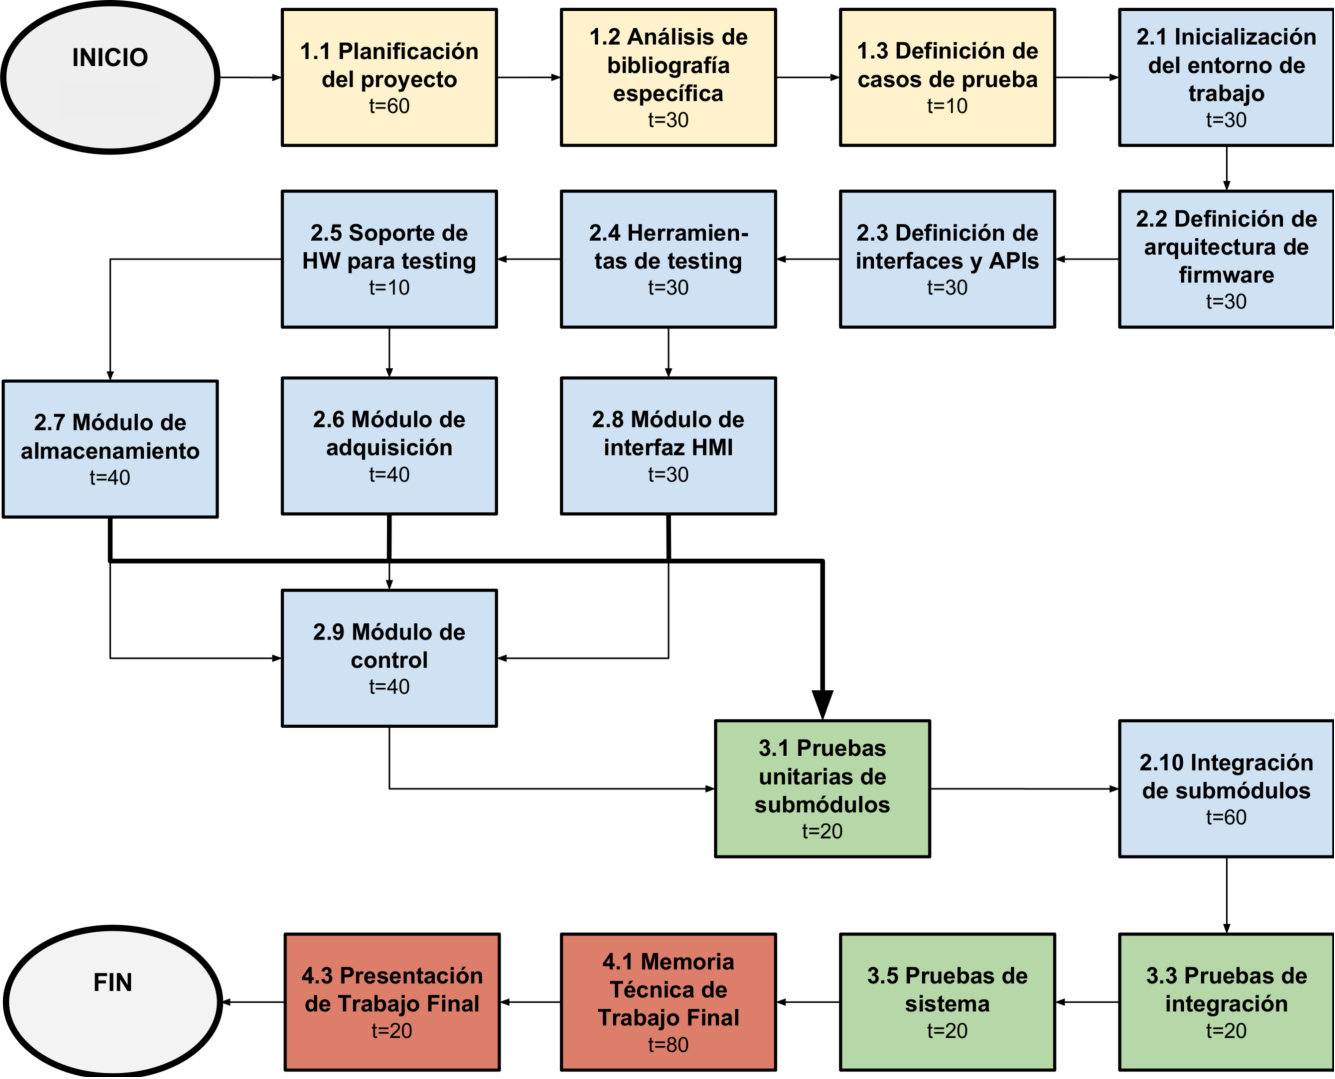
\includegraphics[width=\textwidth]{./Figures/AoN.pdf}
	\caption[Diagrama \textit{Activity on Node}.]{Diagrama \textit{Activity on Node}.  En colores puede distinguirse: en amarillo la etapa de documentación y análisis preliminar; en azul la etapa de diseño e implementación; en verde la etapa de verificación y validación y en rojo el proceso de cierre. El tiempo t está expresado en horas.}
	\label{fig:AoN}
\end{figure}

%\clearpage



\section{Metodología}

En esta sección se describen los aspectos metodológicos relevantes que se aplicaron durante el desarrollo del trabajo.  

\subsection{Control de versiones}
\label{subsec:branching}

Se adoptó un modelo de desarrollo creado por Vincent Driessen llamado ``\textit{A successful Git branching model''} \citep{Driessen}.  El modelo está basado en la herramienta de control de versiones \textit{git} y consiste en un conjunto de procedimientos para ordenar y sistematizar el flujo de trabajo. Este modelo propone utilizar un repositorio considerado a los fines prácticos ``central'' (en git todos los repositorios son idénticos) llamado \textit{origin}.  Todos los desarrolladores trabajan contra este repositorio central con las operaciones típicas de \textit{push} y \textit{pop}.  

Adicionalmente, puede haber intercambios entre los repositorios de los distintos desarrolladores que formen un mismo equipo de trabajo. Estos intercambios pueden visualizarse en la figura \ref{fig:esquema-repos}, donde se esquematizan, por un lado, los posibles flujos de trabajo entre el repositorio \textit{origin} y los distintos desarrolladores, y por el otro, entre los repositorios propios de cada desarrollador. 

\begin{figure}[ht]
	\centering
	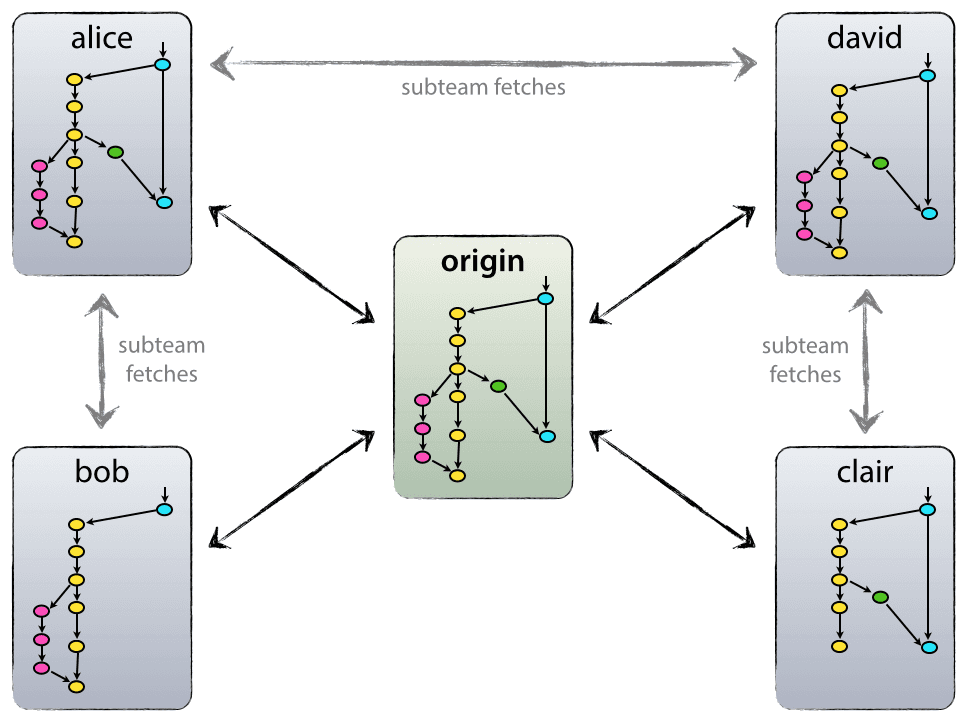
\includegraphics[width=.6\textwidth]{./Figures/centr-decentr@2x.png}
	\caption[Esquema del flujo de trabajo entre repositorios]{Esquema del flujo de trabajo entre repositorios\protect\footnotemark.}
	\label{fig:esquema-repos}
\end{figure}

\footnotetext{Imagen tomada de \url{https://nvie.com/img/centr-decentr@2x.png}.}

Para la elaboración de este trabajo, donde la codificación recayó principalmente sobre una sóla persona, no fueron habituales las operaciones contra un repositorio distinto de \textit{origin}, implementado en \textit{github}. Sin embargo, se considera la experiencia de apropiación de la metodología de trabajo muy valiosa para la formación profesional, ya que el autor de este trabajo no había tenido oportunidad de trabajar tan extensa y sistemáticamente con control de versiones previamente.

En cuanto a la estrategia de uso de ramas, siguiendo el modelo adoptado, se dispuso de dos ramas principales llamadas \textit{master} y \textit{develop}.  En \textit{origin/master} sólo se incluyen \textit{commits} con versiones estables con capacidad de ser puestas en producción, es decir sobre el prototipo de manera que éste pueda operar satisfactoriamente.  En \textit{origin/develop} se encuentran  los últimos cambios que integran las diferentes características ya logradas del código.  Cuando la rama \textit{develop} alcanza un punto de estabilidad y madurez suficiente se debe hacer un \textit{merge} con \textit{master}.% y generar un nuevo número de \textit{release}.

En términos generales, el esquema de ramas propuesto por el modelo de Vincent Driessen puede observar en la figura  \ref{fig:branching} donde se explicitan las posibles interacciones entre ramas.

\vfill

\begin{figure}[!htbp]
	\centering
	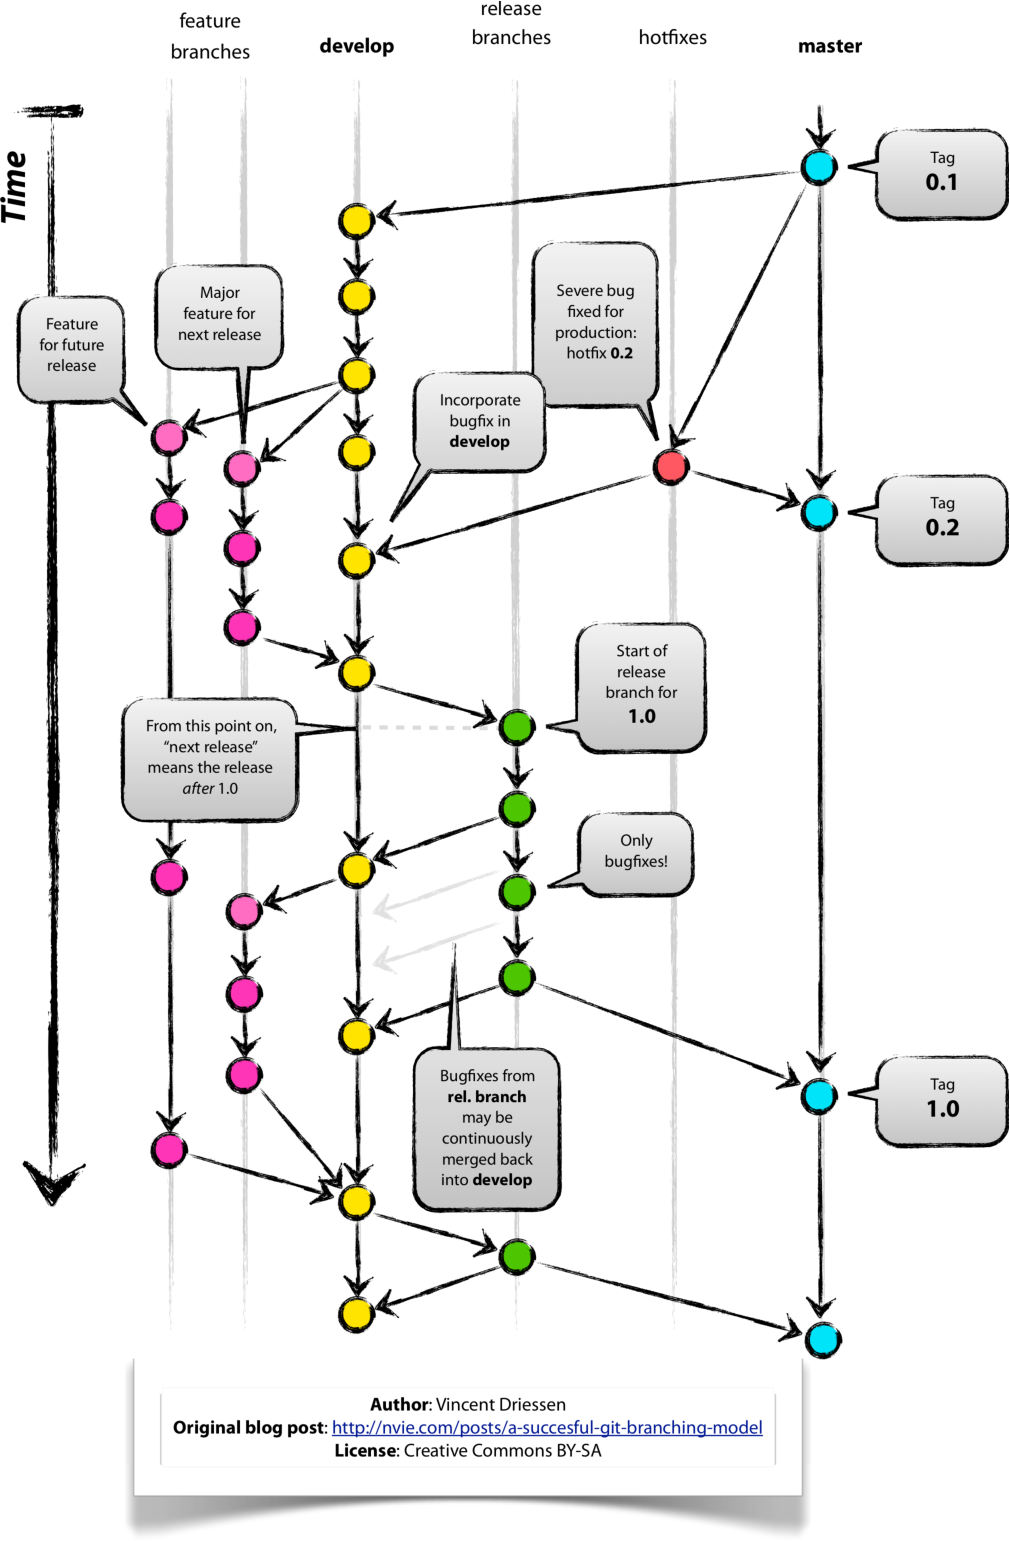
\includegraphics[width=.9\textwidth]{./Figures/Git-branching-model.pdf}
	\caption[Modelo de ramas utilizado en git]{Modelo de ramas utilizado en git\protect\footnotemark.}
	\label{fig:branching}
\end{figure}

\footnotetext{Imagen tomada de \url{https://nvie.com/files/Git-branching-model.pdf}.}

La mecánica de trabajo indica crear una nueva rama por cada característica a implementar.  Cuando la característica se logra, se debe hacer \textit{merge} con la rama \textit{develop} cuidando que no suceda un \textit{fastforward} y se pierdan los \textit{commits} de la rama recién integrada.

Para este trabajo, se crearon ramas para desarrollar cada uno de los subsistemas mencionados en el diagrama en bloques de la figura \ref{fig:diagramaBloquesReducido} e incluidos en el alcance del trabajo, a saber:

\begin{itemize}
	\item \textit{sdcard} para el módulo de almacenamiento.
	\item \textit{onewire} para el módulo de adquisición.
	\item \textit{hmi} para el módulo de interfaz con el usuario.
	\item \textit{control} para el módulo de control.
	\item \textit{ceedling} para el entorno de testing.
\end{itemize}  

\subsection{Paradigma de desarrollo basado en pruebas}
\label{subsec:tdd}

El paradigma de desarrollo basando en pruebas o TDD (por sus siglas en inglés, \textit{Test Driven Development}) \citep{beck2003test} es una práctica de programación que forma parte de las metodologías ágiles.  TDD plantea invertir el orden tradicional de desarrollo en el cual primero de implementa y luego se prueba.  En este sentido, este paradigma propone un proceso de desarrollo que consiste en codificar pruebas, desarrollar y refactorizar de forma iterativa el código.

Si bien no se adoptó el modelo de desarrollo TDD en forma íntegra, sí se incorporaron algunos de sus principios a la metodología de trabajo, en particular los que permiten la producción de un \textit{firmware} modular, altamente reutilizable y preparado para el cambio, es decir escalable, conocidos como principios ``SOLID''\citep{martin2000design}:

\begin{itemize}
	\item Principio de responsabilidad única (\textit{Single responsibility principle}). Cada módulo debe tener una única responsabilidad.
	\item Principio de abierto/cerrado (\textit{Open/closed principle}). Un módulo debe estar abierto para su extensión, pero cerrado para su modificación.
	\item Principio de sustitución de Liskov (\textit{Liskov substitution principle}). Los objetos de un programa deberían ser reemplazables por instancias de sus subtipos sin alterar el correcto funcionamiento del programa.
	\item Principio de segregación de la interfaz (\textit{Interface segregation principle}). Muchas interfaces cliente específicas son mejores que una interfaz de propósito general.
	\item Principio de inversión de la dependencia (\textit{Dependency inversion principle}). Depender de abstracciones, no depender de implementaciones.  Esto significa que un módulo A no debe depender de otro módulo B, sino a través de una abstracción de B.
\end{itemize}

Asimismo, se tomó de TDD la filosofía de pensar primero cómo se va a probar que el código cumple los requerimientos para lograr un mejor entendimiento del sistema y aumentar la calidad del diseño.

En el capítulo \ref{Chapter4} se recopila la documentación de casos de prueba que se usaron como entrada al diseño del \textit{firmware} previo de su implementación.

\subsection{Programación concurrente con Protothreads} 
\label{subsec:protothreads}

Los Protothreads son una abstracción creada por Adam Dunkel para implementar mecanismos de programación concurrente, conocidos como multi-tarea cooperativa, en sistemas embebidos con recursos limitados \citep{Protothreads}. 

Se distribuyen como una biblioteca que puede integrarse al proyecto y posibilitan trabajar con hilos de ejecución sin \textit{stack} o co-rutinas, con mecanismos para bloquear la ejecución de una tarea sin que se produzca un cambio de contexto.  Esto permite un control de flujo secuencial sin máquinas de estado complejas o soporte multi-hilo completo en arquitecturas basadas en eventos \citep{dunkels06protothreads} \citep{dunkels05using}. 

Los protothreads se implementan como un conjunto de macros que el precompilador expande en tiempo de compilación.  

\begin{verbatim}
	struct pt { unsigned short lc; };
	#define PT_THREAD(name_args)  char name_args
	#define PT_BEGIN(pt)          switch(pt->lc) { case 0:
	#define PT_WAIT_UNTIL(pt, c)  pt->lc = __LINE__; \
	                              case __LINE__: \
	                              if(!(c)) return 0
	#define PT_END(pt)            } pt->lc = 0; return 2
	#define PT_INIT(pt)           pt->lc = 0
\end{verbatim}

%\end{lstlisting}
En los algoritmos \ref{lst:proto1} y \ref{lst:proto2} se puede apreciar un ejemplo sencillo que utiliza esta herramienta y el mismo código con las macros expandidas, respectivamente. El \textit{quid} de la implementación es la utlización de una estructura \texttt{switch} y la macro \texttt{\_\_LINE} para insertar el número de línea y permitir la reentrada a una parte del código. En este ejemplo, \texttt{PT\_WAIT\_UNTIL} se encuentra en la línea 12.

\noindent\begin{minipage}{.5\textwidth}
\begin{lstlisting}[caption=Ejemplo de uso,frame=tlrb,basicstyle=\footnotesize,label={lst:proto1}]{Name}
static
PT_THREAD(example(struct pt *pt))
{
  PT_BEGIN(pt);
  
  while(1) {
    PT_WAIT_UNTIL(pt,
      counter == 1000);
    printf("Threshold reached\n");
    counter = 0;
  }
  
  PT_END(pt);
}
\end{lstlisting}
\end{minipage}\hfill
\begin{minipage}{.5\textwidth}
\begin{lstlisting}[caption=Código expandido,frame=tlrb,basicstyle=\footnotesize,label={lst:proto2}]{Name}
static
char example(struct pt *pt)
{
  switch(pt->lc) { case 0:
 
  while(1) {
    pt->lc = 12; case 12:
    if(!(counter == 1000)) return 0;
    printf("Threshold reached\n");
    counter = 0;
  }
 
  } pt->lc = 0; return 2;
}
\end{lstlisting}
\end{minipage}

Se debe tener en cuenta que por la forma en que están implementados, no es posible incluir bloques de control \texttt{switch-case} dentro de los protothreads.	

En el presente trabajo, se hace uso de protothreads en la codificación del protocolo de comunicación 1-wire que se describe en la subsección \ref{subsec:1-wire}.


\section{Arquitectura multicore}
\label{sec:arquitectura}

El \textit{firmware} está desarrollado sobre la base de dos proyectos vinculados dentro IDE MCUXpresso, uno para cada \textit{core} del microcontrolador. Para el IDE, debe haber un proyecto ``maestro'' que controle la ejecución del código (o al menos la secuencia de \textit{startup}) corriendo en el otro \textit{core}, considerado ``esclavo''.  

El proyecto maestro contiene un link al proyecto esclavo que produce que la imagen binaria del esclavo sea incluida en la imagen  binaria del maestro, cuando el proyecto maestro es compilado \citep{nxp:mcuxpresso}. De esta manera, cuando el proyecto maestro es grabado en la flash del microcontrolador, ambos proyectos son descargados a la memoria del microcontrolador.

El proyecto maestro debe ser el que se ejecuta sobre el procesador Cortex-M4 ya que el procesador Cortex-M0 permanece en estado de \textit{reset} hasta que el otro \textit{core} lo libera de este estado escribiendo un 0 en el bit M0SUB\_RST del registro RESET\_CTRL1, como se indica en el manual del microcontrolador \citep{nxp:lpc4337}.

Cuando se energiza el microcontrolador o se produce un \textit{reset}, el \textit{core} maestro inicia su secuencia de \textit{startup} y es responsable de iniciar, a su vez, la secuencia de \textit{startup} del \textit{core} esclavo.  

En las tablas \ref{tab:memoriaM4} y \ref{tab:memoriaM0} se muestra la asignación de bloques de memoria para los procesadores Cortex-M4 y Cortex-M0, respectivamente.  Puede verse que el código de cada procesador se ubica en un bloque de memoria flash independiente, los bancos A y B de 512 kB cada uno.  

Por otra parte, para evitar cualquier tipo de solapamiento en el uso de la RAM, los proyectos asociados a cada \textit{core} se linkean de forma de utilizar exclusivamente bancos de RAM separados.  En este sentido, el procesador cortex-M4 utiliza el primer bloque de RAM de 32 kB y el procesador cortex-M0 utiliza el segundo bloque de RAM de 40kB.

\begin{table}[ht]
\centering
\caption{Asignación de bloques de memoria para el Cortex-M4}
\begin{tabular}{lllll}
\toprule
\textbf{Tipo de memoria} & \textbf{Nombre} & \textbf{Alias} & \textbf{Ubicación} & \textbf{Tamaño} \\ 
\midrule
Flash                    & MFlashA512      & Flash          & 0x1a000000         & 0x80000         \\
RAM                      & RamLoc32        & RAM            & 0x10000000         & 0x8000          \\ 
\bottomrule
\end{tabular}
\label{tab:memoriaM4}
\end{table}

\begin{table}[ht]
\centering
\caption{Asignación de bloques de memoria para el Cortex-M0}
\begin{tabular}{lllll}
\toprule
\textbf{Tipo de memoria} & \textbf{Nombre} & \textbf{Alias} & \textbf{Ubicación} & \textbf{Tamaño} \\ 
\midrule
Flash                    & MFlashB512      & Flash2          & 0x1b000000         & 0x80000         \\
RAM                      & RamLoc40        & RAM2            & 0x10080000         & 0xa000          \\ 
\bottomrule
\end{tabular}
\label{tab:memoriaM0}
\end{table}

Adicionalmente, se define una zona de memoria compartida, visible por ambos procesadores para el intercambio de información. Los mecanismos de comunicación inter-procesadores (IPC, del inglés \textit{Inter Processor Communication}) se describen en la sección \ref{subsec:IPC}. 

\begin{verbatim}
/* Shared memory used by IPC */
#define SHARED_MEM_IPC   0x10088000	 
\end{verbatim}

\subsection{Inter Processor Communications}
\label{subsec:IPC}

Para comunicar ambos procesadores se utiliza una biblioteca provista por el fabricante del microcontrolador NXP, documentada en la nota de aplicación ``AN1117: Inter Processor Communications for LPC43xx'' \citep{nxp:an1117}. En este documento se explican mecanismos posibles para que los dos procesadores intercambien información basados en interrupciones, en colas de mensajes y en ``casillas de correo''.  Este último método queda excluido de esta memoria por no haber sido utilizado en el desarrollo.

\subsubsection{Interrupciones cruzadas}
\label{subsubsec:interrupcion}

El mecanismo de interrupciones cruzadas es el más simple de los tres métodos provistos.  Permite que un \textit{core} active una interrupción en el otro \textit{core} para enviar notificaciones cuya interpretación depende y es exclusiva de la aplicación.  El diseñador puede definir una función de \textit{callback} que es ejecutada en el contexto de la rutina de servicio de la interrupción.  

Para enviar señales al \textit{core} ``remoto'', el \textit{core} ``local'' utiliza una instrucción dedicada SEV (\textit{send event}) provista por la arquitectura Cortex.

Asimismo, dentro de la rutina de interrupción se habilita un \textit{flag} para indicar que se ha recibido una notificación IPC.  Esta variable \textit{flag} puede ser usada por las aplicaciones corriendo sobre el \textit{core} que recibe la notificación para chequear el estado de las comunicaciones. 

La limpieza del \textit{flag} se hace dentro de una sección crítica donde se deshabilitan temporalmente las interrupciones. En el Cortex-M4 se enmascaran las interrupciones con mayor prioridad y en el Cortex-M0 se deshabilitan directamente, ya que este procesador no dispone del mecanismo de enmascaramiento.

El código para generar las interrupciones cruzadas utiliza dos macros. Primero \_\_DSB() (\textit{Data Syncronization Barrier}) para terminar todas las transacciones de memoria pendientes y luego \_\_SEV() (\textit{Send Event}) para generar el envío de una señal de interrupción al otro procesador como puede verse en el algoritmo \ref{lst:ipc_send_signal}.

\begin{lstlisting}[caption={Función ipc\_send\_signal que permite generar una interrupción en el otro procesador.},label={lst:ipc_send_signal}]
/*
 * Initiate interrupt on other processor
 * Upon calling this function generates and interrupt 
 * on the other core. Ex. if called from M0 core it 
 * generates interrupt on M4 core and vice versa.
 */
static void ipc_send_signal(void)
{
  	__DSB();
  	__SEV();
}
\end{lstlisting}

\subsubsection{Colas de mensajes}
\label{subsubsec:colas}

En el método de colas de mensajes, se deben definir dos áreas de memoria compartida, que se utilizan para almacenar los mensajes que cada procesador envía al otro. Una cola (búfer de comandos del \textit{host}) está dedicado a los comandos enviados del procesador maestro al esclavo, y una cola (búfer de mensajes del \textit{host}) se dedica a los mensajes que el procesador esclavo envía en respuesta al procesador maestro. La figura \ref{fig:IPC} muestra esquemáticamente esta configuración.

\vspace{15px}

\begin{figure}[!htpb]
	\centering
	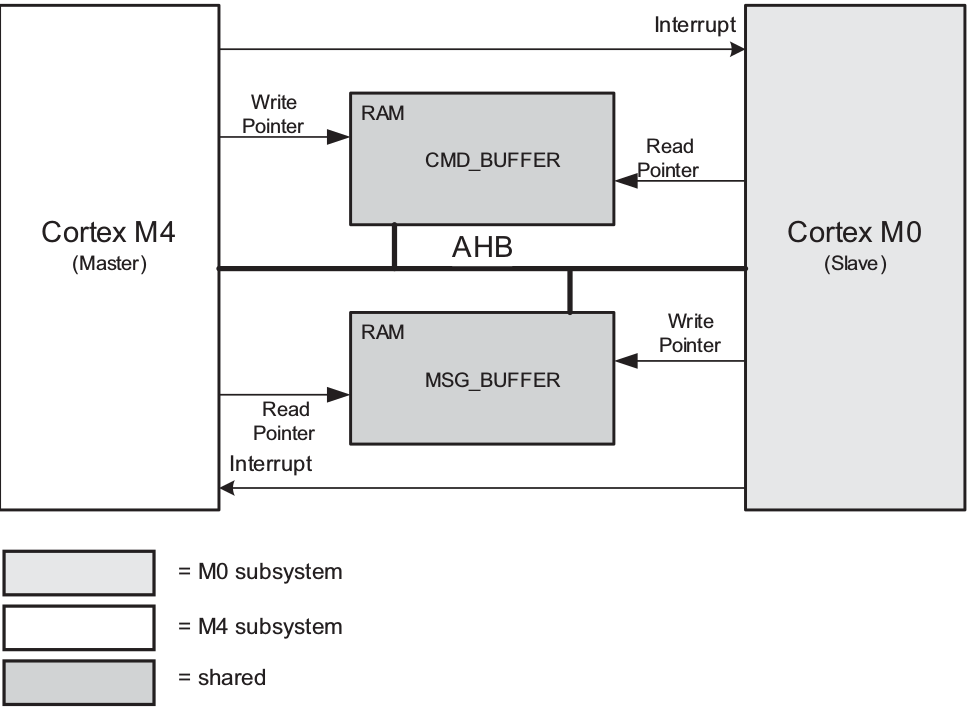
\includegraphics[width=\textwidth]{./Figures/IPC.png}
	\caption[Esquema de comunicación entre procesadores]{Esquema de comunicación entre procesadores basado en colas de mensajes\protect\footnotemark.}
	\label{fig:IPC}
\end{figure}

\vspace{15px}
%\vfill
\footnotetext{Imagen tomada del manual de usuario del microcontrolador LPC4337 \citep{nxp:lpc4337}}

En el esquema propuesto, sólamente el procesador maestro puede escribir en el búfer de comandos y recibe los mensaje del esclavo leyendo el búfer de mensajes.  De manera análoga, únicamente el esclavo puede escribir en el búfer de mensajes y recibe comandos leyendo el búfer de comandos.

Cuando un procesador escribe un nuevo mensaje en una cola, debe notificar al otro procesador de que hay nueva información para procesar. Para tal fin, se utiliza el mecanismo de interrupción descripto en el apartado Interrupciones cruzadas, dentro de la subsección \ref{subsubsec:interrupcion}.

El procesador que recibe el mensaje invoca a un despachador de eventos que busca en un vector de manejadores de eventos el que haya sido registrado para tal fin. En el algoritmo \ref{lst:ipc_dispatcher} se pude apreciar la función provista por la bilbioteca IPC para despachar eventos.

\vspace{10px}

\begin{lstlisting}[caption={Función despachadora de eventos de la biblioteca IPC.},label={lst:ipc_dispatcher}]
/* This task will receive the message from the other 
 * core and will invoke the appropriate callback with
 * the message
 */
static void ipcex_dispatch_task(void *unused)
{
  int ret;
  ipcex_msg_t msg;
  	do {
    	ret = IPC_popMsgTout(&msg, -SYS_OS_ID);
    	if((ret != QUEUE_VALID) || 
                      (msg.id.pid >= IPCEX_MAX_PID)){
      	continue;
    	}
    	if (ipcex_callback_lookup[msg.id.pid]) {
      	ipcex_callback_lookup[msg.id.pid](&msg);
    	}
  	} while (SYS_OS_ID);
}
\end{lstlisting}
\vspace{5px}
SYS\_OS\_ID es una macro que se utiliza para identificar el tipo de Sistema Operativo incluido en la aplicación.  En el caso particular de este trabajo, SYS\_OS\_ID es igual a 0 y esto significa que no hay Sistema Operativo.  Se debe notar que SYS\_OS\_ID = 0 implica que el despachador de eventos se ejecuta una única vez por mensaje recibido.

La función despachadora de eventos descripta en el algoritmo \ref{lst:ipc_dispatcher} fue modificada para adaptarla a las necesitadas del proyecto.  En la sección \ref{sec:control} se documenta cómo se implementó esta función dentro del módulo de control de la estación de monitoreo de ruido acústico.

Para el intercambio de mensajes en el sistema, se define un nuevo tipo de dato \texttt{ipcex\_msg\_t}.  Se trata de una estructura que contiene información que identifica al CPU y al proceso destinararios del mensaje, definidos dentro de otra estructura anidada, junto con dos campos para datos como se observa en el algoritmo \ref{lst:ipcex_msg_t}. 

\begin{lstlisting}[caption={Definición de un nuevo tipo de dato ipcex\_msg\_t para intercambio de mensajes.},label={lst:ipcex_msg_t}]
typedef struct __ipcex_msg {
  struct {
    uint16_t cpu;
    uint16_t pid;
  } id;

  uint32_t data0;
  uint32_t data1;
} ipcex_msg_t;
\end{lstlisting}

El tipo de datos \texttt{ipcex\_msg\_t}, tal como viene definido en la biblioteca IPC fue modificado como se documenta en la sección \ref{sec:control}.
 
\chapter{Diseño e Implementación} % Main chapter title

\label{Chapter3} % Change X to a consecutive number; for referencing this chapter elsewhere, use \ref{ChapterX}
\definecolor{mygreen}{rgb}{0,0.6,0}
\definecolor{mygray}{rgb}{0.5,0.5,0.5}
\definecolor{mymauve}{rgb}{0.58,0,0.82}

\lstset{ %
  backgroundcolor=\color{white},   % choose the background color; you must add \usepackage{color} or \usepackage{xcolor}
  basicstyle=\large,        % the size of the fonts that are used for the code
  breakatwhitespace=false,         % sets if automatic breaks should only happen at whitespace
  breaklines=true,                 % sets automatic line breaking
  captionpos=b,                    % sets the caption-position to bottom
  commentstyle=\color{mygreen},    % comment style
  deletekeywords={...},            % if you want to delete keywords from the given language
  %escapeinside={\%*}{*)},          % if you want to add LaTeX within your code
  %extendedchars=true,              % lets you use non-ASCII characters; for 8-bits encodings only, does not work with UTF-8
  %frame=single,	                   % adds a frame around the code
  keepspaces=true,                 % keeps spaces in text, useful for keeping indentation of code (possibly needs columns=flexible)
  keywordstyle=\color{blue},       % keyword style
  language=[ANSI]C,					% the language of the code
  %otherkeywords={*,...},           % if you want to add more keywords to the set
  numbers=none,                    % where to put the line-numbers; possible values are (none, left, right)
  numbersep=5pt,                   % how far the line-numbers are from the code
  numberstyle=\tiny\color{mygray}, % the style that is used for the line-numbers
  rulecolor=\color{black},         % if not set, the frame-color may be changed on line-breaks within not-black text (e.g. comments (green here))
  showspaces=false,                % show spaces everywhere adding particular underscores; it overrides 'showstringspaces'
  showstringspaces=false,          % underline spaces within strings only
  showtabs=false,                  % show tabs within strings adding particular underscores
  stepnumber=1,                    % the step between two line-numbers. If it's 1, each line will be numbered
  stringstyle=\color{mymauve},     % string literal style
  tabsize=2,	                   % sets default tabsize to 2 spaces
  title=\lstname,                   % show the filename of files included with \lstinputlisting; also try caption instead of title
  morecomment=[s]{/*}{*/}%
}

En este capítulo se presentan la arquitectura multicore del \textit{firmware}, los mecanismos de comunicación entre procesadores y el detalle del diseño de los módulos desarrollados junto con sus interfaces.  Finalmente, se incluye una sección de trazabilidad de requerimientos con las funciones implementadas.

%----------------------------------------------------------------------------------------
%	SECTION 1
%----------------------------------------------------------------------------------------

\section{Arquitectura multicore}
\label{sec:arquitectura}

El \textit{firmware} está desarrollado sobre la base de dos proyectos vinculados del IDE MCUXpresso, uno para cada \textit{core} del microcontrolador. Para el IDE, debe haber un proyecto ``maestro'' que controle la ejecución del código (o al menos la secuencia de \textit{startup}) corriendo en el otro \textit{core}, considerado ``esclavo''.  

El proyecto maestro contiene un link al proyecto esclavo que produce que la imagen binaria del esclavo sea incluida en la imagen  binaria del maestro, cuando el proyecto maestro es compilado \citep{nxp:mcuxpresso}. De esta manera, cuando el proyecto maestro es grabado en la flash del microcontrolador, ambos proyectos son descargados a la memoria del microcontrolador.

El proyecto maestro debe ser el que se ejecuta sobre el procesador Cortex-M4 ya que el procesador Cortex-M0 permanece en estado de \textit{reset} hasta que el otro \textit{core} lo libera de este estado escribiendo un 0 en el bit M0SUB\_RST del registro RESET\_CTRL1, como se indica en el manual del microcontrolador \citep{nxp:lpc4337}.

Cuando se energiza el microcontrolador o se produce un \textit{reset}, el \textit{core} maestro inicia su secuencia de \textit{startup} y es responsable de iniciar, a su vez, la secuencia de \textit{startup} del \textit{core} esclavo.  

En las tablas \ref{tab:memoriaM4} y \ref{tab:memoriaM0} se muestra la asignación de bloques de memoria para los procesadores Cortex-M4 y Cortex-M0, respectivamente.  Puede verse que el código de cada procesador se ubica en un bloque de memoria flash independiente, los bancos A y B de 512 kB cada uno.  

Por otra parte, para evitar cualquier tipo de solapamiento en el uso de la RAM, los proyectos asociados a cada \textit{core} se linkean de forma de utilizar exclusivamente bancos de RAM separados.  En este sentido, el procesador cortex-M4 utiliza el primer bloque de RAM de 32 kB y el procesador cortex-M0 utiliza el segundo bloque de RAM de 40kB.

\begin{table}[ht]
\centering
\caption{Asignación de bloques de memoria para el Cortex-M4}
\begin{tabular}{lllll}
\toprule
\textbf{Tipo de memoria} & \textbf{Nombre} & \textbf{Alias} & \textbf{Ubicación} & \textbf{Tamaño} \\ 
\midrule
Flash                    & MFlashA512      & Flash          & 0x1a000000         & 0x80000         \\
RAM                      & RamLoc32        & RAM            & 0x10000000         & 0x8000          \\ 
\bottomrule
\end{tabular}
\label{tab:memoriaM4}
\end{table}

\begin{table}[ht]
\centering
\caption{Asignación de bloques de memoria para el Cortex-M0}
\begin{tabular}{lllll}
\toprule
\textbf{Tipo de memoria} & \textbf{Nombre} & \textbf{Alias} & \textbf{Ubicación} & \textbf{Tamaño} \\ 
\midrule
Flash                    & MFlashB512      & Flash2          & 0x1b000000         & 0x80000         \\
RAM                      & RamLoc40        & RAM2            & 0x10080000         & 0xa000          \\ 
\bottomrule
\end{tabular}
\label{tab:memoriaM0}
\end{table}

Adicionalmente, se define una zona de memoria compartida, visible por ambos procesadores para el intercambio de información. Los mecanismos de comunicación inter-procesadores (IPC, del inglés \textit{Inter Processor Communication}) se describen en la sección \ref{subsec:IPC}. 

\begin{verbatim}
/* Shared memory used by IPC */
#define SHARED_MEM_IPC   0x10088000	 
\end{verbatim}

\subsection{Inter Processor Communications}
\label{subsec:IPC}

Para comunicar ambos procesadores se utiliza una biblioteca provista por el fabricante del microcontrolador NXP, documentada en la nota de aplicación ``AN1117: Inter Processor Communications for LPC43xx'' \citep{nxp:an1117}. En este documento se explican mecanismos posibles para que los dos procesadores intercambien información basados en interrupciones, en colas de mensajes y en ``casillas de correo''.  Este último método queda excluido de esta memoria por no haber sido utilizado en el desarrollo.

\subsubsection{Interrupciones cruzadas}
\label{subsubsec:interrupcion}

El mecanismo de interrupciones cruzadas es el más simple de los 3 métodos provistos.  Permite que un \textit{core} active una interrupción en el otro \textit{core} para enviar notificaciones cuya interpretación depende y es exclusiva de la aplicación.  El diseñador puede definir una función de \textit{callback} que es ejecutada en el contexto de la rutina de servicio de la interrupción.  

Para enviar señales al \textit{core} ``remoto'', el \textit{core} ``local'' utiliza una instrucción dedicada SEV (\textit{send event}) provista por la arquitectura Cortex.

Asimismo, dentro de la rutina de interrupción se habilita un \textit{flag} para indicar que se ha recibido una notificación IPC.  Esta variable \textit{flag} puede ser usada por las aplicaciones corriendo sobre el \textit{core} que recibe la notificación para chequear el estado de las comunicaciones. 

La limpieza del \textit{flag} se hace dentro de una sección crítica donde se deshabilitan temporalmente las interrupciones. En el Cortex-M4 se enmascaran las interrupciones con mayor prioridad y en el Cortex-M0 se deshabilitan directamente, ya que este procesador no dispone del mecanismo de enmascaramiento.

El código para generar las interrupciones cruzadas utiliza dos macros. Primero \_\_DSB() (\textit{Data Syncronization Barrier}) para terminar todas las transacciones de memoria pendientes y luego \_\_SEV() (\textit{Send Event}) para generar el envío de una señal de interrupción al otro procesador como puede verse en el algoritmo \ref{lst:ipc_send_signal}.
%, como puede apreciarse en \ref{cod:interrupt}
%\begin{verbatim}
%/*
% * Initiate interrupt on other processor
% * Upon calling this function generates and interrupt 
% * on the other core. Ex. if called from M0 core it 
% * generates interrupt on M4 core and vice versa.
% */
%static void ipc_send_signal(void)
%{
%  	__DSB();
%  	__SEV();
%}
%\end{verbatim}\label{cod:interrupt}  

\begin{lstlisting}[caption={Función ipc\_send\_signal que permite generar una interrupción en el otro procesador.},label={lst:ipc_send_signal}]
/*
 * Initiate interrupt on other processor
 * Upon calling this function generates and interrupt 
 * on the other core. Ex. if called from M0 core it 
 * generates interrupt on M4 core and vice versa.
 */
static void ipc_send_signal(void)
{
  	__DSB();
  	__SEV();
}
\end{lstlisting}

\subsubsection{Colas de mensajes}
\label{subsubsec:colas}

En el método de colas de mensajes, se deben definir dos áreas de memoria compartida, que se utilizan para almacenar los mensajes que cada procesador envía al otro. Una cola (búfer de comandos del \textit{host}) está dedicado a los comandos enviados del procesador maestro al esclavo, y una cola (búfer de mensajes del \textit{host}) se dedica a los mensajes que el procesador esclavo envía en respuesta al procesador maestro. La figura \ref{fig:IPC} muestra esquemáticamente esta configuración.

\vspace{10px}

\begin{figure}[ht]
	\centering
	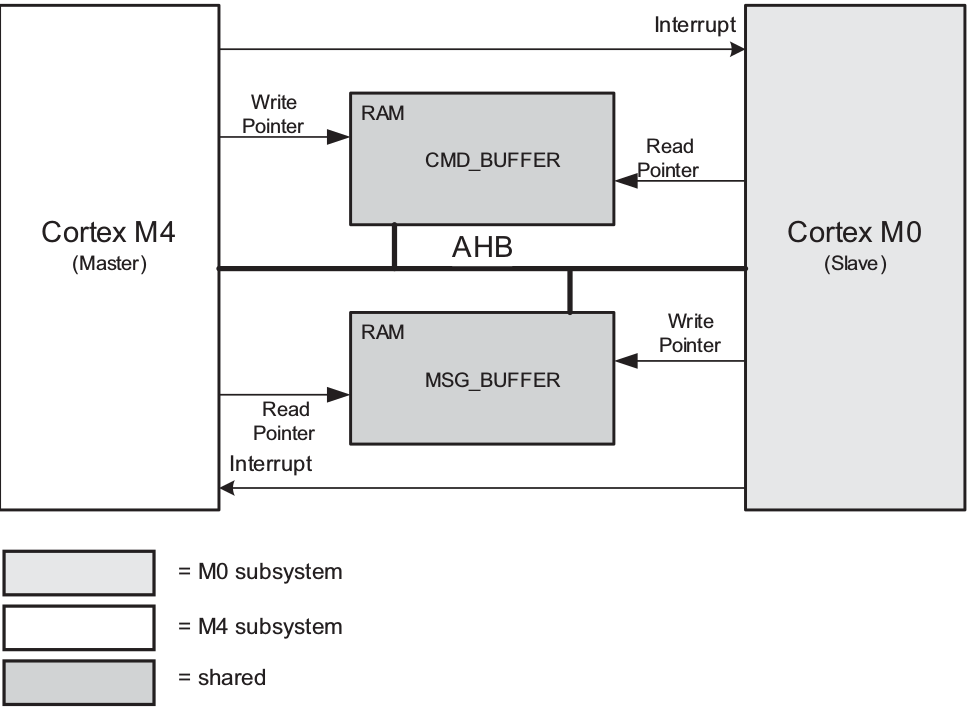
\includegraphics[width=.8\textwidth]{./Figures/IPC.png}
	\caption[Esquema de comunicación entre procesadores]{Esquema de comunicación entre procesadores basado en colas de mensajes\protect\footnotemark.}
	\label{fig:IPC}
\end{figure}

\vspace{10px}
\vfill
\footnotetext{Imagen tomada del manual de usuario del microcontrolador LPC4337 \citep{nxp:lpc4337}}

En el esquema propuesto, sólamente el procesador maestro puede escribir en el búfer de comandos y recibe los mensaje del esclavo leyendo el búfer de mensajes.  De manera análoga, únicamente el esclavo puede escribir en el búfer de mensajes y recibe comandos leyendo el búfer de comandos.

Cuando un procesador escribe un nuevo mensaje en una cola, debe notificar al otro procesador de que hay nueva información para procesar. Para tal fin, se utiliza el mecanismo de interrupción descrito en el apartado Interrupciones cruzadas, dentro de la subsección \ref{subsubsec:interrupcion}.  Luego de esto, el procesador que recibe el mensaje invoca a un despachador de eventos que busca en un vector de manejadores de eventos el que haya sido registrado para tal fin. En el algoritmo \ref{lst:ipc_dispatcher} se pude apreciar la función provista por la bilbioteca IPC para despachar eventos.

\vspace{10px}

\begin{lstlisting}[caption={Función despachadora de eventos de la biblioteca IPC.},label={lst:ipc_dispatcher}]
/* This task will receive the message from the other 
 * core and will invoke the appropriate callback with
 * the message
 */
static void ipcex_dispatch_task(void *unused)
{
  int ret;
  ipcex_msg_t msg;
  	do {
    	ret = IPC_popMsgTout(&msg, -SYS_OS_ID);
    	if((ret != QUEUE_VALID) || 
                      (msg.id.pid >= IPCEX_MAX_PID)){
      	continue;
    	}
    	if (ipcex_callback_lookup[msg.id.pid]) {
      	ipcex_callback_lookup[msg.id.pid](&msg);
    	}
  	} while (SYS_OS_ID);
}
\end{lstlisting}
\vspace{5px}
SYS\_OS\_ID es una macro que se utiliza para identificar el tipo de Sistema Operativo incluido en la aplicación.  En el caso particular de este trabajo, SYS\_OS\_ID es igual a 0 y esto significa que no hay Sistema Operativo.  Se debe notar que SYS\_OS\_ID = 0 implica que el despachador de eventos se ejecuta una única vez por mensaje recibido.

La función despachadora de eventos descrita en el algoritmo \ref{lst:ipc_dispatcher} fue modificada para adaptarla a las necesitadas del proyecto.  En la sección \ref{sec:control} se documenta cómo se implementó esta función dentro del módulo de control de la estación de monitoreo de ruido acústico.

Para el intercambio de mensajes en el sistema, se define un nuevo tipo de dato \texttt{ipcex\_msg\_t}.  Se trata de una estructura que contiene información que identifica al CPU y al proceso destinararios del mensaje, definidos dentro de otra estructura anidada, junto con dos campos para datos como se observa en el algoritmo \ref{lst:ipcex_msg_t}. 

\begin{lstlisting}[caption={Definición de un nuevo tipo de dato ipcex\_msg\_t para intercambio de mensajes.},label={lst:ipcex_msg_t}]
typedef struct __ipcex_msg {
  struct {
    uint16_t cpu;
    uint16_t pid;
  } id;

  uint32_t data0;
  uint32_t data1;
} ipcex_msg_t;
\end{lstlisting}

El tipo de datos \texttt{ipcex\_msg\_t}, tal como viene definido en la biblioteca IPC fue modificado como se documenta en la sección \ref{sec:control}.

\section{Diseño de módulos y definición de interfaces}
\label{sec:modulos}

El optó por un diseño fuertemente modularizado en archivos, junto a un modelo de capas jerárquicas para organizar el código en distintos niveles de abstracción.  

En la figura \ref{fig:capas} se pueden observar, agrupados por color, las capas utilizadas en este trabajo.  En color amarillo, el paquete de drivers provistos por el fabricante del silicio; en color naranja la capa de bibiotecas; la capa de abstracción de \textit{hardware} (HAL, por sus siglas en inglés) en color verde; y finalmente, en color celeste, la capa de aplicación con los cuatro módulos implementados.   

%\vspace{10px}

\begin{figure}[ht]
	\centering
	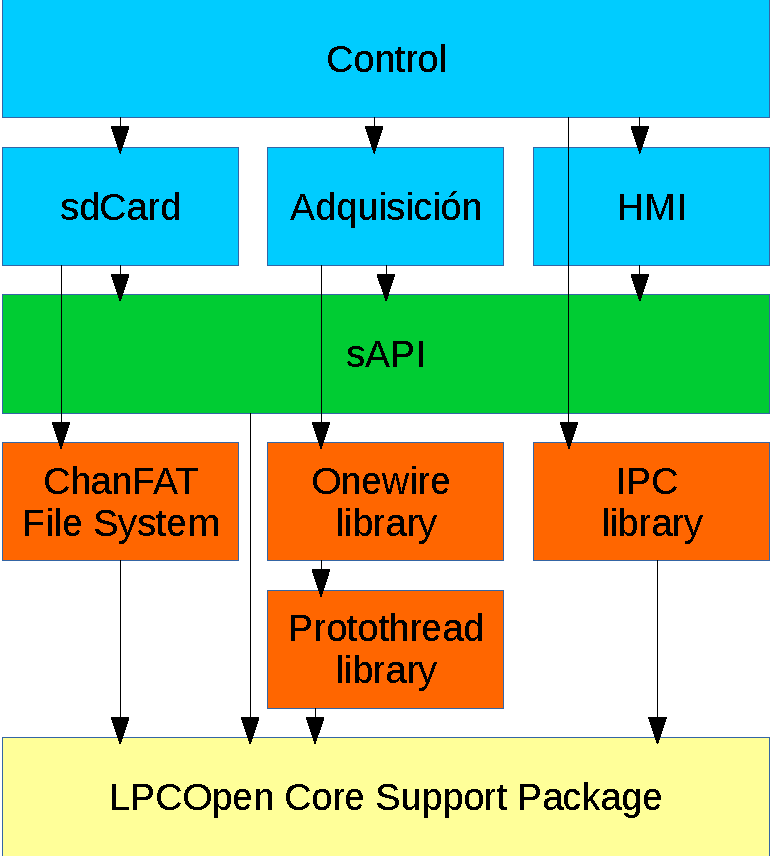
\includegraphics[width=.5\textwidth]{./Figures/capas.pdf}
	\caption[Estructura de capas para el \textit{firmware}.]{Estructura de capas para el \textit{firmware}. En orden creciente de nivel de abstracción: \textit{core support package} (amarillo), bibliotecas (naranja), sAPI (verde) y la capa de aplicación (celeste) con los 4 módulos implementados.}
	\label{fig:capas}
\end{figure}

\vspace{10px}

Para los módulos en la capa de aplicación, se confeccionó una matriz de trazabilidad de los requerimientos referidos al firmware, detallados en la sección \ref{sec:requerimientos}. 

La tabla \ref{tab:trazabilidad} permite saber en qué módulo del firmware serán implementados los requerimientos funcionales del proyecto.  Asimismo, permite controlar que todo este subconjunto de requerimientos sea implementado y que no haya superposición entre la funcionalidad de cada módulo.

\vspace{5px}

\begin{table}[ht]
\caption[Matriz de trazabilidad de requerimientos funcionales]{Matriz de trazabilidad de requerimientos funcionales con los módulos de \textit{firmware}}
\label{tab:trazabilidad}
\begin{tabular}{lcccc}
\toprule
\textbf{Requerimiento} & \textbf{Control} & \textbf{sdCard} & \textbf{Adquisición} & \textbf{HMI} \\ \midrule
2.1 Adquirir temperatura                   &                  &                 & X                    &              \\ %\hline
2.2 Adquirir velocidad de viento           &                  &                 & X                    &              \\ %\hline
2.3 Almacenar datos                        &                  & X               &                      &              \\ %\hline
2.4 Perfiles de consumo                    & X                &                 &                      &              \\ %\hline
2.5 Interfaz                               &                  &                 &                      & X            \\ \bottomrule
\end{tabular}
\end{table}

Se definió un nuevo tipo de dato, \texttt{module\_t} que contiene campos de control para los módulos. Se observa su la definición el el algoritmo \ref{lst:module_t}.

El primer campo de \texttt{module\_t} indica en qué procesador debe ejecutarse el módulo. Sigue un campo para identificar al módulo y un puntero a la función manejadora de eventos que será invocada cada vez que haya un mensaje para este módulo. Para temporizar en forma periódica la ejecución del módulo se utiliza el campo \texttt{period} y, finalmente, se incluye un campo para el estado del módulo que puede tomar uno de los siguientes valores: DISABLE, READY o PROCESSING.

\vspace{10px}

\begin{lstlisting}[caption={Definición de un nuevo tipo de dato module\_t.},label={lst:module_t}]
typedef struct {
   CPUID_T coreID;
   moduleID_t moduleID;
   funcPtr_t eventHandler;
   tick_t period;
   moduleStatus_t status;
} module_t;
\end{lstlisting}

\vspace{10px}

Toda la interacción con los módulos se realiza a través de los respectivos manejadores de eventos y una cola de mensajes como la descrita en la subsección \ref{subsubsec:colas}. Para el intercambio de mensajes entre módulos que se encuentren en ejecución en un mismo procesador, se levantaron las restricciones de escritura sobre la propia cola de mensajes que se originalmente pesaban sobre cada procesador.

A continuación se listan los prototipos de los manejadores de eventos definidos:

\vspace{10px}

\begin{itemize}
  \item \texttt{void onewire\_handler(const ipcex\_msg\_t * msg );} 
  \item \texttt{void hmi\_handler(const ipcex\_msg\_t * msg );} 
  \item \texttt{void sdcard\_handler(const ipcex\_msg\_t * msg );} 
  \item \texttt{void control\_handler(const ipcex\_msg\_t * msg );} 
\end{itemize}

\vspace{10px}

Puede notarse que todos los manejadores reciben un mismo tipo de parámetro, un puntero constante a un mensaje de tipo \texttt{ipcex\_msg\_t}.  Cada módulo es responsable de interpretar los dos campos enteros sin signo de 32 bits de datos que contiene el mensaje.  Normalmente el campo \texttt{data0} define un comando y \texttt{data1} se utiliza opcionalmente para el envío de parámetros.

Para todos los módulos se utilizó un modelo de \textit{firmware} basado en máquinas de estados finitos (MEF) jerárquicas, donde una MEF principal controla la lógica de funcionamiento con el mayor nivel de abstracción. Los diferentes estados, a su vez, pueden o no estar modelados con MEFs dependiendo de la conveniencia de esto último.

Se definió una arquitectura de máquia de estados finitos principal lo más genérica posible de forma que pueda ser compartida por los distintos módulos.  En este sentido, todos los módulos poseen un estado \texttt{DISABLE}, \texttt{INIT}, \texttt{IDLE}, \texttt{CONFIG} y \texttt{CHECK}. La funcionalidad que implemente cada uno de estos estados será propia del módulo donde estén definidos. 

Todos los módulos inician en estado \texttt{DISABLE}. Adicionalmente, la máquina de estados finitos podrá tener otros estados que sean específicos para lograr sus propósitos funcionales.

En la figura \ref{fig:mef_generica} se muestra un diagrama de la máquina de estados finitos genérica, diseñada para ser usada como base en cada uno de los módulos que componen el sistema.

\begin{figure}[htpb]
	\centering
	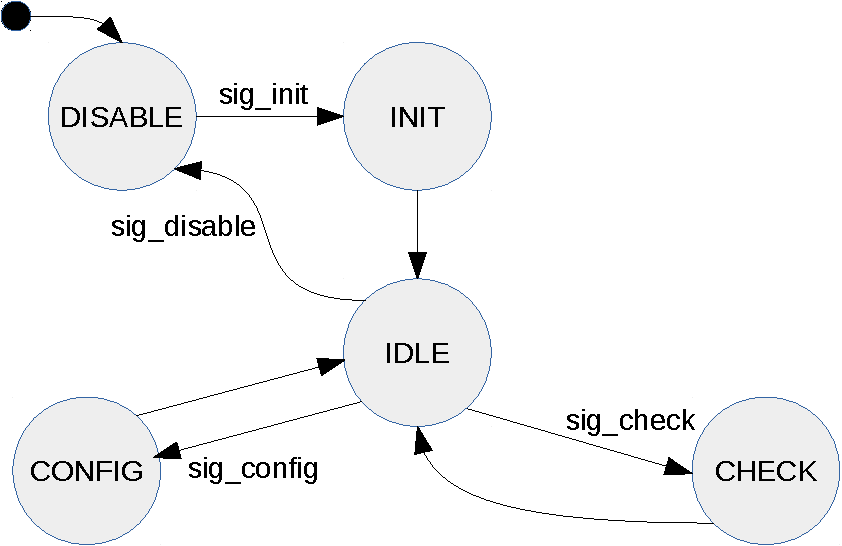
\includegraphics[width=\textwidth]{./Figures/MEF_generica.pdf}
	\caption[Diseño de MEF genérica para los módulos]{Diseño de máquina de estados finitos genérica para el control de la lógica de los módulos}
	\label{fig:mef_generica}
\end{figure}

\section{Módulo de almacenamiento}
\label{sec:almacenamiento}

El propósito del módulo de almacenamiento es proveer al sistema de una interfaz para operar con un medio de almacenamiento no volátil que permita guardar en forma permanente los datos registrados por el módulo de adquisición y eventualmente un log con información de \textit{debug}.  

\subsection{Medio físico}
\label{subsec:mediofisico}

Se evaluaron distintas opciones de medios físicos.  En la tabla \ref{tab:medios} se recopilan las alternativas analizadas y se especifica un orden de magnitud para la capacidad de almacenamiento posible, el tipo de interfaz con el microcontrolador y el protocolo que debe implementarse en el \textit{firmware} para su utilización.

\vspace{10px}

\begin{table}[ht]
\centering
\caption{Alternativas de medios físicos evaluados.}
\label{tab:medios}
\begin{tabular}{lrcc}
\toprule
\multicolumn{1}{c}{\textbf{Medio físico}} & \multicolumn{1}{c}{\textbf{Capacidad}} & \textbf{Interfaz} & \textbf{Protocolo} \\ \midrule
USB Mass Storage Device                   & $\sim$10 Gb                            & USB 2.0           & USB                \\
Tarjeta de memoria microSD                & $\sim$10 Gb                            & Micro SD          & SSP                \\
Disco de estado sólido (SSD)              & $\sim$100 Gb                           & SATA III          & SATA               \\
Disco duro mecánico (HHD)                 & $\sim$1000 Gb                          & SATA III          & SATA               \\ \bottomrule
\end{tabular}
\end{table}

\vspace{10px}

Teniendo en cuenta criterios de costos y simplicidad de interacción con la CIAA-NXP, se decidió utilizar un lector de tarjetas microSD con comunicación sobre un puerto \textit{Synchronous Serial Port} (SSP).  Este protocolo es compatible con el protocolo SPI y utiliza un bus de 4 cables con las señales SCK, SSEL, MISO y MOSI.  Asimismo, el soporte seleccionado minimiza el consumo de energía comparado con las otras alternativas, lo cual lo hace deseable para la aplicación.  

El lector de tarjetas utilizado se presenta en la figura \ref{fig:lector_sdCard}, donde puede verse esquemáticamente el diagrama de conexionado eléctrico entre la CIAA-NXP y el lector (figura \ref{fig:lector_conexionado}) y una vista superior del módulo de hardware (figura \ref{fig:lector_hardware}). Cabe notar que al haber un único dispositivo ``escalvo'' en el bus SSP, la señal de \textit{chip select} (CS) se conecta con GND, lo que implica que el dispositivo está permanente seleccionado.

\vspace{20px}

\begin{figure}[h]
	\centering
	\begin{subfigure}{.4\textwidth}
		\centering
		\begin{tabular}{rll}
			\textbf{CIAA-NXP }&	& \textbf{Lector de tarjetas}\\
			+3.3V     & --\textgreater{} & +3.3V   \\
			GND       & --\textgreater{} & CS  \\
			SPI\_MOSI & --\textgreater{} & MOSI  \\
			SPI\_SCK  & --\textgreater{} & SCK \\
			SPI\_MISO & --\textgreater{} & MISO  \\
			GND       & --\textgreater{} & GND  \\
		\end{tabular}
		\caption{ }
  		\label{fig:lector_conexionado}
	\end{subfigure}%
	\begin{subfigure}{.6\textwidth}
	\hspace{15px}
		\centering
		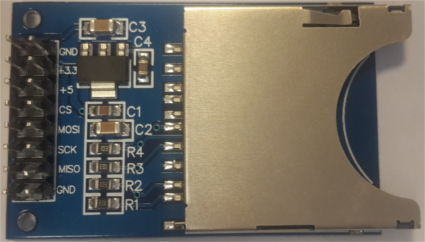
\includegraphics[height=3.3cm]{./Figures/sdCardReader.jpg}
		\caption{ }
		\label{fig:lector_hardware}
	\end{subfigure}
	\caption{(A) Diagrama de conexionado eléctrico y (B) Lector de tarjetas SD utilizado.}
	\label{fig:lector_sdCard}
\end{figure}

\vspace{10px}

Para la utilización del lector de tarjetas se hizo uso de la biblioteca FatFs, desarrollada por chaN \citep{fatFS}. FatFs es un módulo de sistema de archivos FAT/exFAT genérico para sistemas embebidos limitados en recursos. En la figura \ref{fig:chan} se esquematizan las interfaces de la biblioteca en una aplicación típica. 

\begin{figure}[htpb]
	\centering
	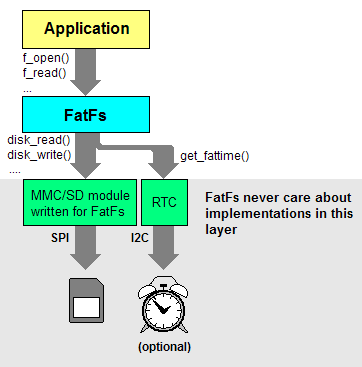
\includegraphics[width=.5\textwidth]{./Figures/chan.png}
	\caption[Diagrama de capas de fatFs]{Diagrama de capas con la ubicación de la biblioteca fatFs en el sistema y sus interfaces\protect\footnotemark.}
	\label{fig:chan}
\end{figure}

\footnotetext{Imagen tomada de \url{http://elm-chan.org/fsw/ff/doc/appnote.html}.}

El código está escrito en ANSI C y es \textit{software} libre bajo licencia estilo BSD \citep{BSD}.

\subsection{Máquina de Estados Finitos}
\label{subsec:MEFsdcard}

Se presenta el diagrama de estado de la MEF principal del módulo en la figura \ref{fig:mef_sdcard}, donde puede apreciase el punto de entrada con un circulo negro, los estado que puede tomar la máquina y las señales que provocan los cambios de estado. Se omiten del gráfico las salidas del sistema por simplicidad. 

Debe notarse que al energizarse el sistema o luego de un \textit{reset}, el módulo se encuentra deshabilitado, con la MEF en el estado \texttt{DISABLE}, del cual sólo puede salir si se recibe una señal de inicialización.  

Una vez inicializado, el módulo se encontrará la mayor parte del tiempo en el estado \texttt{IDLE} a la espera de un comando válido.  

Cuando el módulo esté realizando alguna operación de lectura, escritura o actualización sobre la tarjeta SD, el estado del módulo tendrá el valor \texttt{PROCESSING} para indicarle al módulo de control que debe tener acceso a tiempo de CPU para poder completar las operaciones pendientes.  

Todas las operación del módulo desde que es inicializado terminan incondicionalmente en el estado \texttt{IDLE}, en donde el valor de la variable que registra el estado del módulo cambia de \texttt{PROCESSING} a \texttt{READY}.

\begin{figure}[htpb]
	\centering
	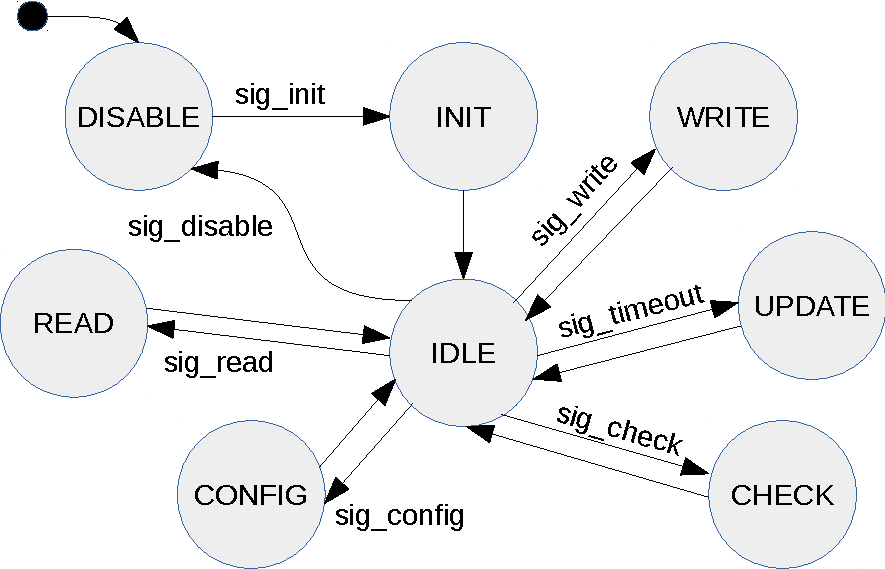
\includegraphics[width=\textwidth]{./Figures/MEF_sdCard_2.pdf}
	\caption[MEF principal del módulo de almacenamiento sdCard]{Máquina de estados finitos principal del módulo de almacenamiento.}
	\label{fig:mef_sdcard}
\end{figure}

%  Se indican las señales que puede recibir junto con las acciones más relevantes de cada estado. principal del módulo de almacenamiento

En la tabla \ref{tab:estadosAlmacenamiento} se describen los posibles estados de la MEF junto con las señales para alcanzarlos. Asimismo se explicitan las acciones y actividades más destacables que se realizan en cada uno de ellos.

% Please add the following required packages to your document preamble:
% \usepackage{graphicx}
\begin{table}[htpb]
\centering
\caption[Descripción de los estados de la MEF principal del módulo de almacenamiento.]{Descripción de los estados de la MEF principal del módulo de almacenamiento.}
\label{tab:estadosAlmacenamiento}
\resizebox{\textwidth}{!}{%
\begin{tabular}{lll}
\toprule
\multicolumn{1}{c}{\textbf{Estado}} & \multicolumn{1}{c}{\textbf{Señal para cambio}} & \multicolumn{1}{c}{\textbf{Acciones y actividades}} \\ \midrule
DISABLE & Reset o sig\_disable & \begin{tabular}[c]{@{}l@{}}Desinicializar el controlador SPI.\\ Desinicializar la bilioteca fatFS.\\ Desinicializar el módulo de almacenamiento.\\ Cambiar el estado del módulo de READY a DISABLE.\end{tabular} \\
 &  &  \\
INIT & sig\_init & \begin{tabular}[c]{@{}l@{}}Inicializar el controlador SPI.\\ Inicializar la bilioteca fatFS.\\ Inicializar el módulo de almacenamiento.\\ Cambiar el estado del módulo de DISABLE a READY.\end{tabular} \\
 &  &  \\
IDLE & transición incondicional & Cambiar estado del módulo de PROCESSING a READY. \\
 &  &  \\
CONFIG & sig\_config & Realizar cambios de configuración al módulo. \\
 &  &  \\
CHECK & sig\_check & Realizar autochequeo e informar al módulo de control \\
 &  &  \\
UPDATE & sig\_timeout & Ejecutar tarea periódica de actualización de la tarjeta SD. \\
 &  &  \\
WRITE & sig\_write & Obtener timestamp y escribir datos en la tarjeta SD. \\
 &  &  \\
READ & sig\_read & Leer datos en la tarjeta SD \\ \bottomrule
\end{tabular}%
}
\end{table}


\clearpage
\section{Módulo de adquisición}
\label{sec:adquisicion}

El propósito del módulo de adquisición es proveer al sistema de una interfaz para operar los distintos sensores que puedan conectarse a la estación.  Originalmente, se contempló el uso de uno o varios termómetros y un anemómetro para medir temperatura del agua y velocidad del viento en superficie, respectivamente. Adicionalmente, se contempla incorporar hidrofónos para registrar el nivel de ruido submarino, principal objetivo de la estación de medición.

Se mencionó en la sección \ref{sec:objetivosyalcances}, que los hidrófonos quedaron fuera del alcance del proyecto en esta etapa del desarrollo.  De igual manera, el control del anemómetro quedará fuera de la implementación ya que se optó por priorizar el requerimiento implícito de cumplir con la fecha de entrega.  Se retoma este punto en el capítulo \ref{Chapter5}, en la sección \ref{subsec:metasalcanzadas}, donde se discuten sus implicancias.

Sin pérdida de generalidad, la arquitectura de módulo adoptada puede utilizarse para incorporar los sensores no implementados, en una segunda iteración.

\subsection{Sensor de temperatura}
\label{subsec:1-wire}

%En la presente sección se presenta la implementación del control para el sensor de temperatura. 

Se evaluaron distintas opciones para el sensor de temperatura que estuvieran disponibles en el mercado local.  Se recopila en la tabla \ref{tab:temperatura} la información relevada para los sensores candidatos, donde puede verse fabricante y modelo de cada dispositivo junto con las principales características de interés para la aplicación.

Cabe destacar que la limitante para el rango de temperatura no es el propio sensor sino el plástico que recubre los hilos conductores que lo conectan al microcontrolador, motivo por el cual todas las alternativas evaluadas poseen rangos equivalente.  Se utiliza en la tabla un código sencillo para indicar un orden de magnitud del costo relativo del sensor con \$ para costo bajo, \$\$ para costo medio y \$\$\$ para costo alto.

% Please add the following required packages to your document preamble:
% \usepackage{graphicx}
\begin{table}[htpb]
\centering
\caption{Alternativas de sensor de temperatura evaluadas.}
\label{tab:temperatura}
\resizebox{\textwidth}{!}{%
\begin{tabular}{ccccccc}
\toprule
\textbf{Fabricante} & \textbf{Sensor} & \textbf{Tipo} & \textbf{Precisión (\grados C)} & \textbf{Rango (\grados C)} & \textbf{Interfaz} & \textbf{Costo} \\
\midrule
Maxim Integrated    & DS18B20     & Termómetro digital & $\pm$ 0.5 & -55 a +125   & 1-wire & \$             \\
\multicolumn{1}{l}{} & \multicolumn{1}{l}{} & \multicolumn{1}{l}{} & \multicolumn{1}{l}{} & \multicolumn{1}{l}{} & \multicolumn{1}{l}{} & \multicolumn{1}{l}{} \\
Genérico            & IM120628010 & Termistor NTC & 1\% & -25 a +125   & 1-wire & \$             \\
\multicolumn{1}{l}{} & \multicolumn{1}{l}{} & \multicolumn{1}{l}{} & \multicolumn{1}{l}{} & \multicolumn{1}{l}{} & \multicolumn{1}{l}{} & \multicolumn{1}{l}{} \\
Texas Instruments         & LM35  & Integrated Circuit & $\pm$ 0.5 & -55 a +150   & \textit{Analog}         & \$   \\
\multicolumn{1}{l}{} & \multicolumn{1}{l}{} & \multicolumn{1}{l}{} & \multicolumn{1}{l}{} & \multicolumn{1}{l}{} & \multicolumn{1}{l}{} & \multicolumn{1}{l}{} \\
Altas Scientific    & PT-1000A    & \begin{tabular}[c]{@{}c@{}}RTD \\ (resistance\\ temperature\\ detector)\end{tabular} & $\pm$ (0.15 + 0.002*t)  & -55 a +125   & \textit{Analog}         & \$\$\$         \\
\bottomrule         
\end{tabular}%
}
\end{table}

El sensor elegido es el termómetro digital DS18B20 del fabricante Maxim Integrated \citep{ds18b20}. Los motivos de la elección fueron principalmente la facilidad de uso en un entorno embebido de recursos limitados, la disponibilidad de documentación completa y detallada junto con numerosas notas de aplicación y el bajo costo del dispositivo.

En la figura \ref{fig:ds18b20_bloques} se puede apreciar un diagrama en bloques del sensor, en donde destaca la interfaz de 3 cables con una línea bidireccional de datos (DQ) y dos cables para la alimentación (GND y $V_{DD}$). 

El sensor admite una configuración de alimentación ``parásita'', en la cual se energiza desde la línea de datos DQ, lo que habilita a prescindir de un cable a costa de mayores requerimientos para la temporización de las comunicaciones y la utilización de un transistor a modo de \textit{``strong pull-up''} (conectado el bus de datos directamente a $V_{DD}$).

\begin{figure}[htpb]
	\centering
	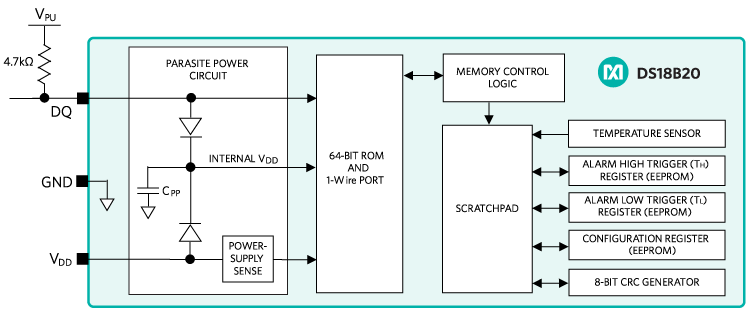
\includegraphics[width=.8\textwidth]{./Figures/ds18b20_bloques.png}
	\caption[Diagrama en bloques del sensor de temperatura DS18B20]{Diagrama en bloques del sensor de temperatura\protect\footnotemark.}
	\label{fig:ds18b20_bloques}
\end{figure}

\footnotetext{Imagen tomada de \url{https://www.maximintegrated.com/en/images/qv/2812.png}}

Cada sensor posee un código de identificación único de 64 bits que permite operar con múltiples sensores sobre un mismo bus de tipo 1-wire.  Mediante un algoritmo de descubrimiento se pueden identificar los sensores conectados a un mismo bus y controlarlos independientemente. 

La capacidad para identificar cuántos sensores hay conectados en cada momento y poder interrogarlos individualmente se utilizó para incorporar una funcionalidad de autochequeo, en la cual el microcontrolador es capaz de detectar si un sensor ha dejado de funcionar correctamente.

Otras características destacables son la posibilidad de configurar la resolución entre 9 y 12 bits, el uso de CRC en las comunicaciones y la capacidad para definir umbrales de alarma para los valores de temperatura medidos.

Este sensor se comercializa con distintas longitudes de cable, dentro de un encapsulado metálico sumergible.  Para este trabajo se adquirieron dos sensores sumergibles con 5 metros de cable y 2 metros de cable, respectivamente.   

Los dos sensores operan sobre una misma línea de datos con una resistencia de \textit{pull-up} de 2,2 K$\Omega$, como puede verse en el diagrama de conexionado eléctrico de la figura \ref{fig:ds18b20_conexionado}.  El encapsulado sumergible puede apreciarse en la figura \ref{fig:termometro}.

%\vspace{10px}

\begin{figure}[htpb]
	\centering
	\begin{subfigure}{.6\textwidth}
		\centering
		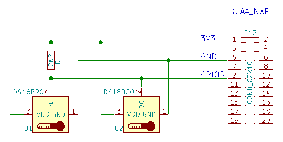
\includegraphics[height=3.7cm]{./Figures/ds18b20_conexionado.pdf}
		\caption{ Diagrama de conexionado eléctrico}
  		\label{fig:ds18b20_conexionado}
	\end{subfigure}%
	\begin{subfigure}{.4\textwidth}
		\centering
		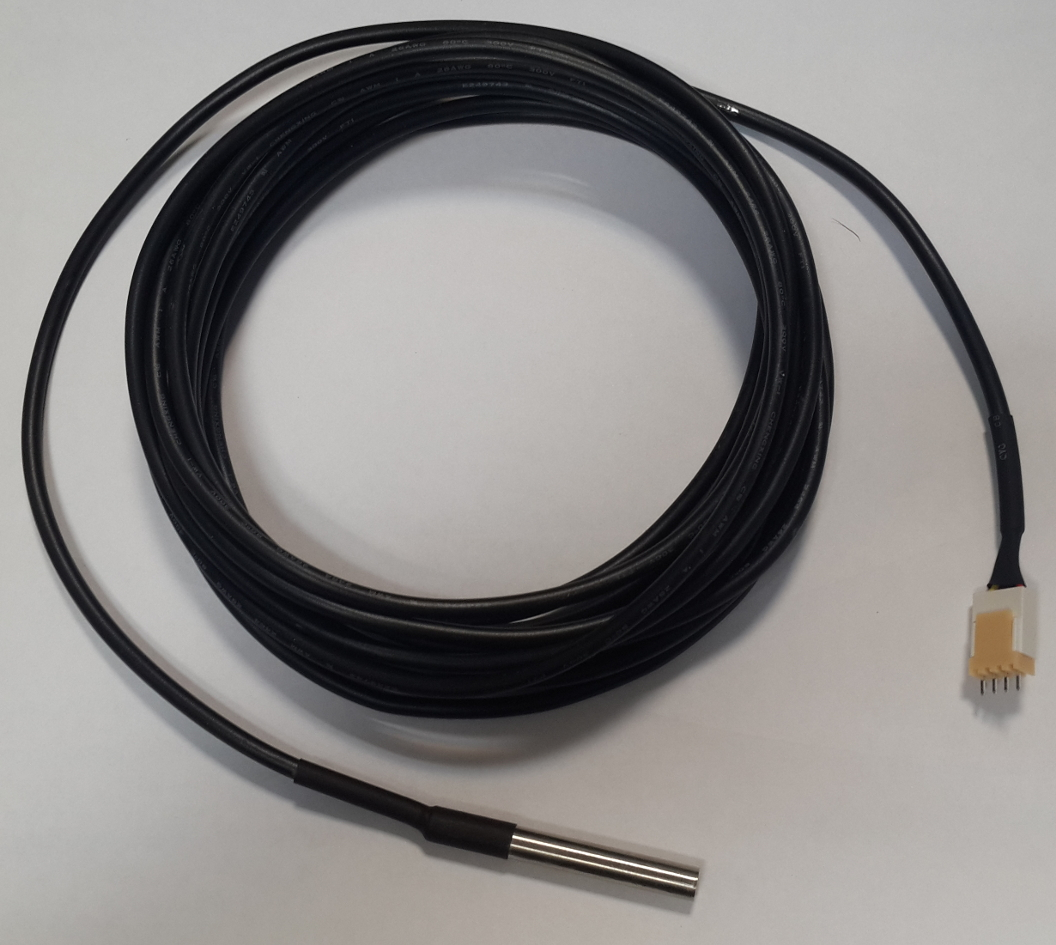
\includegraphics[height=3.7cm]{./Figures/ds18b20.jpg}
		\caption{ Sensor DS18B20}
		\label{fig:termometro}
	\end{subfigure}
	\caption{}
	\label{fig:ds18b20}
\end{figure}


Para el control de los dispositivos se adaptó una implementación de controlador de bus \textit{1-wire} para microcontroladores de la familia LPC1343, desarrollada en forma de biblioteca por James Harwood \citep{harwood}.  En esta biblioteca se hace uso de las técnicas de programación concurrente descritas en el capitulo \ref{Chapter2}, subsección \ref{subsec:protothreads}.

\subsection{Máquina de Estados Finitos}

En forma análoga a lo presentado en la subsección \ref{subsec:MEFsdcard}, se muestra aquí el diagrama de estado de la MEF principal del módulo en la figura \ref{fig:mef_adquisicion}, donde puede apreciase el punto de entrada con un circulo negro, los estado que puede tomar la máquina y las señales que provocan los cambios de estado. Se omiten del gráfico las salidas del sistema por simplicidad. 

Igualmente, debe notarse que cuando el sistema es energizado o luego de un \textit{reset}, el módulo se encuentra deshabilitado, con la MEF en el estado \texttt{DISABLE}, del cual sólo puede salir si se recibe una señal de inicialización.  

Una vez inicializado, el módulo se encontrará la mayor parte del tiempo en el estado \texttt{IDLE} a la espera de un comando válido.  

Cuando el módulo esté realizando alguna operación de adquisición, configuración o autochequeo sobre los sensores conectados, el estado del módulo tendrá el valor \texttt{PROCESSING} para indicarle al módulo de control que debe tener acceso a tiempo de CPU para poder completar las operaciones pendientes.  

Todas las operación del módulo desde que es inicializado terminan incondicionalmente en el estado \texttt{IDLE}, en donde el valor de la variable que registra el estado cambia de \texttt{PROCESSING} a \texttt{READY}.

\begin{figure}[htpb]
	\centering
	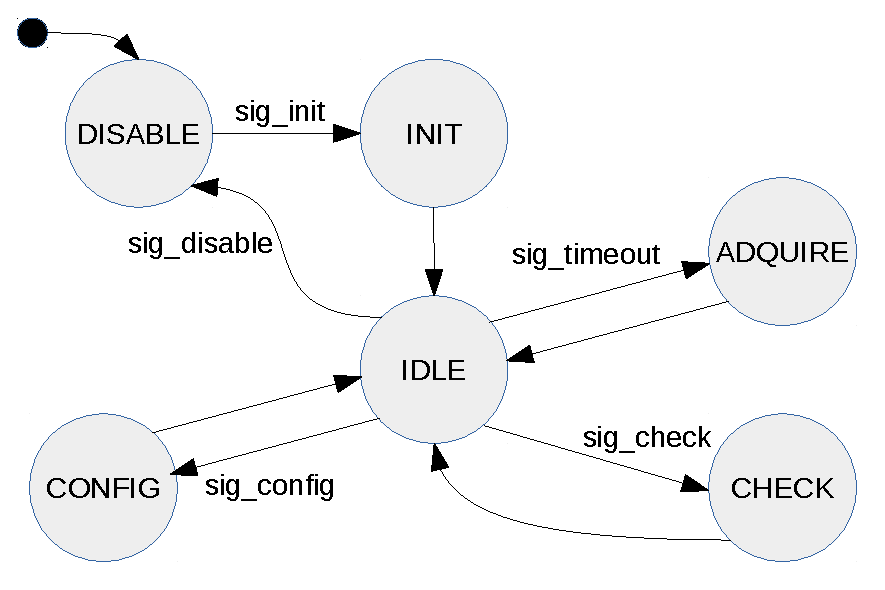
\includegraphics[width=\textwidth]{./Figures/MEF_adquisicion.pdf}
	\caption[MEF principal del módulo de adquisición de temperatura]{Máquina de estados finitos principal del módulo de adquisición de temperatura}
	\label{fig:mef_adquisicion}
\end{figure}

Las principales acciones y actividades de cada estado se describen en la tabla \ref{tab:estadosAdquisicion}.  Asimismo, se indican las señales válidas que puede recibir la MEF junto con las transiciones que éstas provocan.

% Please add the following required packages to your document preamble:
% \usepackage{graphicx}
\begin{table}[htpb]
\centering
\caption[Descripción de los estados de la MEF principal del módulo de adquisición.]{Descripción de los estados de la MEF principal del módulo de adquisición.  Se indican las señales que puede recibir junto con las acciones más relevantes de cada estado.}
\label{tab:estadosAdquisicion}
\resizebox{\textwidth}{!}{%
\begin{tabular}{lll}
\toprule
\multicolumn{1}{c}{\textbf{Estado}} & \multicolumn{1}{c}{\textbf{Señal para cambio}} & \multicolumn{1}{c}{\textbf{Acciones y actividades}} \\ \midrule
DISABLE & Reset o sig\_disable & \begin{tabular}[c]{@{}l@{}}Desinicializar el TIMER0.\\ Deshabilitar la interrupción TIMER0\_IRQn. \\ Desinicializar el GPIO 3[0].\\ Cambiar el estado del módulo de READY a DISABLE.\end{tabular} \\
 &  &  \\
INIT & sig\_init & \begin{tabular}[c]{@{}l@{}}Inicializar el TIMER0.\\ Habilitar la interrupción TIMER0\_IRQn.\\ Inicializar el GPIO3[0].\\ Cambiar el estado del módulo de DISABLE a READY.\end{tabular} \\
 &  &  \\
IDLE & transición incondicional & Cambiar estado del módulo de PROCESSING a READY. \\
 &  &  \\
CONFIG & sig\_config & Realizar cambios de configuración al módulo. \\
 &  &  \\
CHECK & sig\_check & Realizar autochequeo e informar al módulo de control \\
 &  &  \\
ADQUIRE & sig\_timeout & Ejecutar tarea periódica de adquisición de datos \\ \bottomrule
\end{tabular}%
}
\end{table}
%\subsection{Sensor de velocidad de viento}
%\label{subsec:anemometro}

\section{Módulo interfaz máquina-hombre}
\label{sec:HMI}

El propósito del módulo interfaz máquina-hombre (HMI, por sus siglas en inglés) es proveer al sistema de un medio de interacción con un operador humano. Las posibles interacciones se realizan a través de una interfaz de comandos interactiva y contempla operaciones de configuración y cambio de parámetros sobre los módulos y operaciones de mantenimiento y depuración del sistema.  

La interfaz se implementa desde el microcontrolador sobre un puerto serie de tipo \textit{Universal Asynchronous Receiver-Transmitter} o UART a través de un conversor RS232/USB de la firma FTDI incorporado en la CIAA-NXP, hasta llegar finalmente a la PC del operador humano.

El código del módulo incluye directivas de compilación condicional que permiten cambiar la cantidad y el nivel de detalle de los mensajes que el sistema envía a través de la interfaz.  Esta opción debe definirse en tiempo de compilación y no puede ser modificada en tiempo de ejecución, es decir, una vez que el sistema esté en funcionamiento  

Mediante la definición de una MACRO en el archivo \texttt{board\_api.h}:
\begin{verbatim}
  #define DEBUG_ENABLE
\end{verbatim}

\noindent se habilitan funciones de depuración que envían mensajes a través de la UART como puede verse en el algorirmo \ref{lst:debug}.  

Adicionalmente, si se define la MACRO \texttt{DEBUG\_SEMIHOSTING} se pueden utilizar los recursos de entrada/salida de la PC host que esté depurando el sistema embebido. 

Si la MACRO \texttt{DEBUG\_ENABLE} no es definida, las funciones no se incluyen en el código, ahorrando recursos al sistema.

\vspace{10px}

\begin{lstlisting}[caption={Macros para habilitar/deshabilitar mensajes de depuración del código.},label={lst:debug}]
#if defined(DEBUG_ENABLE)

  #if defined(DEBUG_SEMIHOSTING)
	  
    #define DEBUGINIT()
    #define DEBUGOUT(...) printf(__VA_ARGS__)
    #define DEBUGSTR(str) printf(str)
    #define DEBUGIN() (int) EOF

  #else
  
    #define DEBUGINIT() Board_Debug_Init()
    #define DEBUGOUT(...) printf(__VA_ARGS__)
    #define DEBUGSTR(str) Board_UARTPutSTR(str)
    #define DEBUGIN() Board_UARTGetChar()
  
  #endif /* defined(DEBUG_SEMIHOSTING) */

#else
  
  #define DEBUGINIT()
  #define DEBUGOUT(...)
  #define DEBUGSTR(str)
  #define DEBUGIN() (int) EOF
  
#endif /* defined(DEBUG_ENABLE) */
\end{lstlisting}

Para acceder a la interfaz se debe utilizar una terminal serie tipo \texttt{screen} \citep{screen} en configuración 8N1 a 115200 baudios. 

Existen emuladores de terminales serie como \textit{cutecom}, de gran difusión, que presentan el inconveniente de no implementar funciones de control definidas en los estándares ANSI X3.64 (ISO 6429) e ISO 2022 por lo que la visualización de la interfaz en estas consolas puede ser defectuosa y no se recomienda su uso.


\subsection{Interfaz}
\label{subsec:interfaz}

El propósito de la interfaz desarrollada es servir como prueba de concepto e incluye un mínimo de funcionalidad para cumplir los requerimientos relacionados a la controlabilidad de la estación, principalmente en lo referido al período de muestreo de los sensores del módulo de adquisición. 

Cabe destacar que el valor de esta interfaz no está en su estética ni en su facilidad de uso, sino en la arquitectura subyacente que permite obtener información sistema y operar sobre sus distintos componentes.

Una primera versión de la interfaz operativa se presenta en la figura \ref{fig:interfaz_main}, donde pueden apreciarse 4 zonas funcionales identificadas con recuadros de color rojo, a saber: encabezado, menú de opciones, línea de comandos y barra de estado. 

\begin{figure}[htpb]
	\centering
	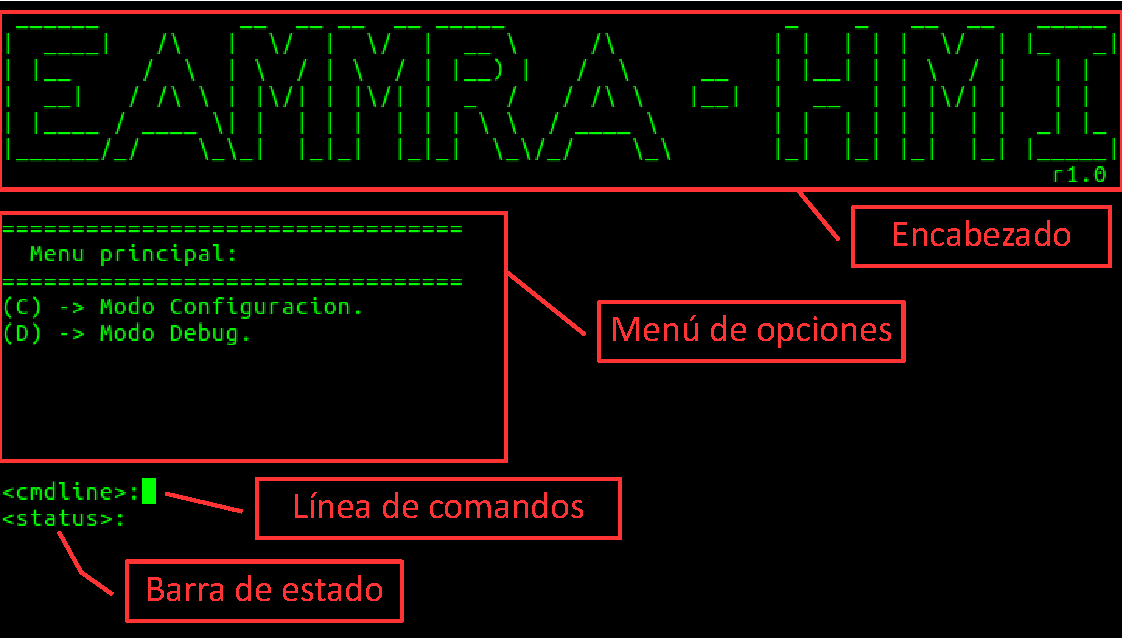
\includegraphics[width=\textwidth]{./Figures/interfaz_detalles.pdf}
	\caption[]{Vista de la pantalla principal de la interfaz. Se destacan con recuadros rojos 4 secciones dentro de la pantalla: encabezado, menú de opciones, línea de comandos y barra de estado.}
	\label{fig:interfaz_main}
\end{figure}

En el encabezado puede observarse el nombre de la estación EAMMRA, por las siglas de ``Estación Autónoma Marítima de Medición de Ruido Ambiente'' junto en una identificación del número de revisión de la interfaz, en el caso de la figura \ref{fig:interfaz_main}, r1.0. 

En la zona asociada al menú de opciones se presentan los comandos que puede introducir el operador. En cada pantalla, las opciones que se muestran cambian según el contexto.

Se realiza un eco de los comandos ingresados, que aparecen en la línea de comandos para confirmación del usuario. Asimismo, si se ingresa un caracter que no sea parte de las opciones disponibles, el sistema lo informa a continuación del eco con el mensaje `` no es un comando valido.'' 

Los diferentes módulos pueden enviar mensajes para el usuario que aparecerán en la sección indicada como barra de estado.  De igual manera, cuando el sistema requiera confirmación por parte del usuario, se exhibirá un mensaje para tal fin en esta sección.

Desde el menú principal se puede acceder al modo configuración para interactuar directamente con los módulos del sistema.  Se presenta la pantalla principal de este modo en la figura \ref{fig:interfaz_config}.  Para acceder a las opciones de un módulo en particular se debe ingresar el número asociado a éste en el menú de opciones.  A excepción de la pantalla principal, todas las pantallas cuentan con una opción (X) para volver al menú anterior.

\begin{figure}[htpb]
	\centering
	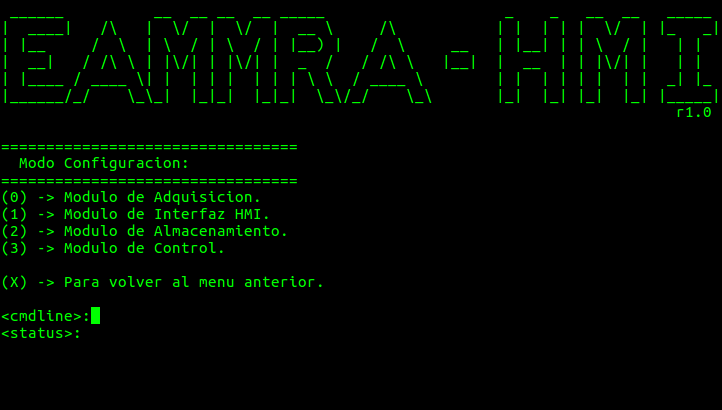
\includegraphics[width=\textwidth]{./Figures/interfaz_config.png}
	\caption[]{Vista de la pantalla principal del modo configuración de la interfaz máquina-hombre.}
	\label{fig:interfaz_config}
\end{figure}

Sin pérdida de generalidad, ya que todos los módulos comparten las mismas opciones, se presenta en la figura \ref{fig:interfaz_config_detalle} una vista de detalle de la pantalla de configuración del módulo de adquisición, también llamado módulo 1-WIRE por el tipo de sensor que controla. Se puede observar la opción de configuración elegida en la línea de comandos y el pedido de confirmación en la barra de estado.

Se contempla diferenciar a futuro las opciones de cada módulo acorde se agregue funcionalidad a los mismos. Las opciones actualmente disponibles son las siguientes:

\begin{itemize}
  \item \texttt{(D)} Habilitar / Deshabilitar: permite intercambiar el estado del módulo entre \texttt{READY} y \texttt{DISABLED}.  Para tal fin, si el módulo se encuentra en estado \texttt{READY}, se le envía una señal sig\_disable.  En caso que se encuentre en estado \texttt{DISABLED} se le envía una señal sig\_init.  Antes de enviar la señal correspondiente se informa al usuario el estado actual del módulo y se pide que confirme o cancele la operación mediante el ingreso de \texttt{`s'} o \texttt{`n'}, respectivamente.
  \item \texttt{(I)} Info del modulo: muestra el estado actual del módulo en la barra de estado.  Las respuestas posibles son \texttt{READY}, \texttt{PROCESSING} y \texttt{DISABLED}
  \item \texttt{(C)} Configurar: permite cambiar la configuración del módulo.  En esta etapa del desarrollo se implementó únicamente la posibilidad de cambiar el tiempo con que se ejecuta la tarea periódica, si la hubiera.
  \item \texttt{(A)} Autocomprobación: permite realizar una comprobación interna de funcionamiento mediante el envío de una señal sig\_check al módulo. En esta etapa del desarrollo la funcionalidad está implementada con una función \textit{mock} que devuelve un mensaje en la barra de estado. 
  \item \texttt{(X)} para volver al menú anterior: cambia el menú a la pantalla principal del modo configuración.
\end{itemize}

\begin{figure}[htpb]
	\centering
	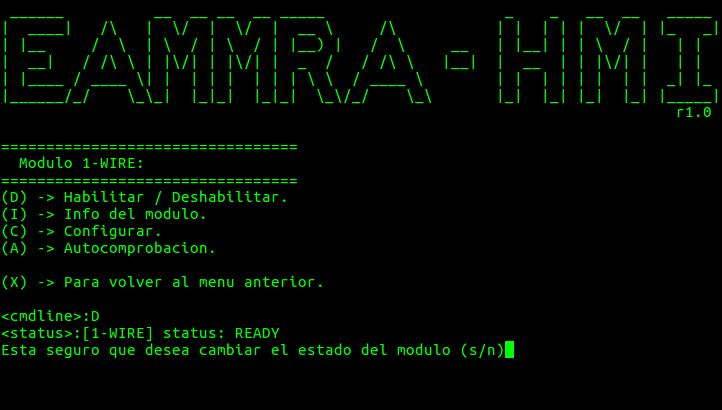
\includegraphics[width=\textwidth]{./Figures/interfaz_config_detalle.png}
	\caption[Pantalla de configuración del módulo de adquisición.]{Pantalla de configuración del módulo de adquisición con una operación de deshabilitación en curso.} 
	\label{fig:interfaz_config_detalle}
\end{figure}

Asimismo, desde el menú principal se puede acceder a un modo \textit{debug} con opciones de depuración y mantenimiento como puede observarse en la figura \ref{fig:interfaz_debug}.  

\begin{figure}[htpb]
	\centering
	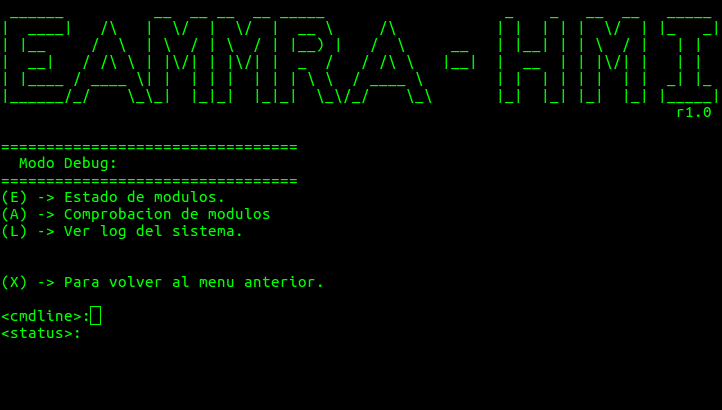
\includegraphics[width=\textwidth]{./Figures/interfaz_debug.png}
	\caption{Vista de la pantalla principal del modo debug de la interfaz máquina-hombre.}
	\label{fig:interfaz_debug}
\end{figure}

Las opciones para este modo son:

\begin{itemize}
  \item \texttt{(E)} Estado de modulos: muestra el estado actual de todos los módulo del sistema en la barra de estado.
  \item \texttt{(A)} Comprobación: permite realizar una comprobación interna de funcionamiento a todos los módulos. En esta etapa del desarrollo la funcionalidad está implementada con una función \textit{mock} que devuelve un mensaje en la barra de estado y registra los resultados en el log del sistema.
  \item \texttt{(L)} Ver log del sistema: permite realizar un \textit{dump} del log del sistema en la consola.  Esto significa que se imprime en la terminal serie todo el contenido del archivo de log ubicado en la tarjeta de memoria microSD. Presionando cualquier tecla se limpia la pantalla y se vuelve al menú principal del modo \textit{debug}.
  \item \texttt{(X)} para volver al menú anterior: cambia el menú a la plantalla principal del modo \textit{debug}.
\end{itemize}

En la tabla \ref{tab:interfaz_config}, se recopilan los comandos que se pueden ingresar por la interfaz en el modo configuración junto con una descripción de la funcionalidad que activa en el sistema.  Asimismo, se explicita si la función se encuentran implementada o maquetada. 

\begin{table}[htpb]
\centering
\caption{Opciones disponibles en el modo configuración de la interfaz.  Se indica el comando para seleccionar la opción y si ésta se encuentra implementada o maquetada.}
\label{tab:interfaz_config}
%\resizebox{\textwidth}{!}{%
\begin{tabular}{ccccc}
\toprule
\textbf{\textbf{Opción}} & \textbf{Descripción} & \textbf{Implementada} & \textbf{Maquetada} \\ \midrule
D & \begin{tabular}[c]{@{}c@{}}Habilitar / Deshabilitar el módulo.\\ Se informa el estado actual\\ Se pide confirmación del usuario\end{tabular} & X &  \\
\multicolumn{1}{l}{} & \multicolumn{1}{l}{} & \multicolumn{1}{l}{} & \multicolumn{1}{l}{} \\
I & Informa el estado del módulo. & X &  \\
\multicolumn{1}{l}{} & \multicolumn{1}{l}{} & \multicolumn{1}{l}{} & \multicolumn{1}{l}{} \\
C & \begin{tabular}[c]{@{}c@{}}Configurar el módulo\\ Permite cambiar el valor de\\ period dentro de la estructura\\ de control del módulo\end{tabular} & X &  \\
\multicolumn{1}{l}{} & \multicolumn{1}{l}{} & \multicolumn{1}{l}{} & \multicolumn{1}{l}{} \\
A & \begin{tabular}[c]{@{}c@{}}Autocomprobación del módulo.\\ Informa en la barra de estado\\ el resultado de la verificación.\end{tabular} &  & X \\ \bottomrule
\end{tabular}%
%}
\end{table}

En forma análoga, se presenta en la tabla \ref{tab:interfaz_debug}, una recopilación de los comandos que se pueden ingresar en el modo debug junto con una descripción de la misma.  Asimismo, se explicita si la función se encuentran implementada o maquetada. 

\begin{table}[htpb]
\centering
\caption{Opciones disponibles en el modo debug de la interfaz.  Se indica el comando para seleccionar la opción y si ésta se encuentra implementada o maquetada.}
\label{tab:interfaz_debug}
%\resizebox{\textwidth}{!}{%
\begin{tabular}{cccc}
\toprule
\textbf{Opción} & \textbf{Descripción} & \textbf{Implementada} & \textbf{Maquetada} \\ \midrule
E & \begin{tabular}[c]{@{}c@{}}Informa el estado actual\\ de todos los módulos \\ en la barra de estado\end{tabular} & X &  \\
\multicolumn{1}{l}{} & \multicolumn{1}{l}{} & \multicolumn{1}{l}{} & \multicolumn{1}{l}{} \\
A & \begin{tabular}[c]{@{}c@{}}Autocomprobación\\ de todos los módulos.\\ Se registra el resultado\\ en el log del sistema\end{tabular} &  & X \\
\multicolumn{1}{l}{} & \multicolumn{1}{l}{} & \multicolumn{1}{l}{} & \multicolumn{1}{l}{} \\
L & \begin{tabular}[c]{@{}c@{}}Listar el contenido del \\ log del sistema.\\ Se limpia presionando\\ cualquier tecla\end{tabular} & X & \\
\bottomrule 
\end{tabular}
%}
\end{table}

En los módulos que tiene funciones maquetadas se reemplazó la llamada a la función que debería realizar la implementación por el envío de un mensaje generado en el propio módulo hacia la interfaz HMI.  De esta manera se puede comprobar el correcto funcionamiento de la interfaz y el circuito de  comunicación entre módulos, es decir, que:

\begin{itemize}
	\item el comando es correctamente recibido por la interfaz,
	\item la interfaz envía correctamente una señal al módulo correspondiente,
	\item el módulo correspondiente recibe la señal y contesta con un mensaje que se visualiza en la barra de estado de la interfaz.
\end{itemize}

Se contempla incluir en versiones futuras, además de cambios estilísticos, la implementación completa de funcionalidades que en la presente versión se encuentran maquetadas.  Si bien estás y otras características son deseable para la usabilidad de la interfaz y la operación de la estación, no formaban parte de los requerimientos enumerados en la sección \ref{sec:requerimientos}. 



\subsection{Máquina de estados finitos}

El diagrama de estado de la MEF principal del módulo puede apreciarse en la figura \ref{fig:mef_HMI}, donde se observa el punto de entrada con un circulo negro, los estados que puede tomar la máquina y las señales que provocan los cambios de estado. Se omiten del gráfico las salidas del sistema por simplicidad. 

Igualmente, debe notarse que cuando el sistema es energizado o luego de un \textit{reset}, el módulo se encuentra deshabilitado, con la MEF en el estado \texttt{DISABLE}, del cual sólo puede salir si se recibe una señal de inicialización.  

Una vez inicializado, el módulo se encontrará la mayor parte del tiempo en el estado \texttt{IDLE} a la espera de un comando válido para procesar.  

Cuando el módulo esté realizando alguna operación de procesamiento de comandos recibidos por el usuario, configuración o autochequeo, el estado en la del módulo tendrá el valor \texttt{PROCESSING} para indicarle al módulo de control que debe tener acceso a tiempo de CPU para poder completar las operaciones pendientes.  

Todas las operación del módulo desde que es inicializado terminan incondicionalmente en el estado \texttt{IDLE}, en donde el valor de la variable que registra el estado cambia de \texttt{PROCESSING} a \texttt{READY}.

\begin{figure}[htpb]
	\centering
	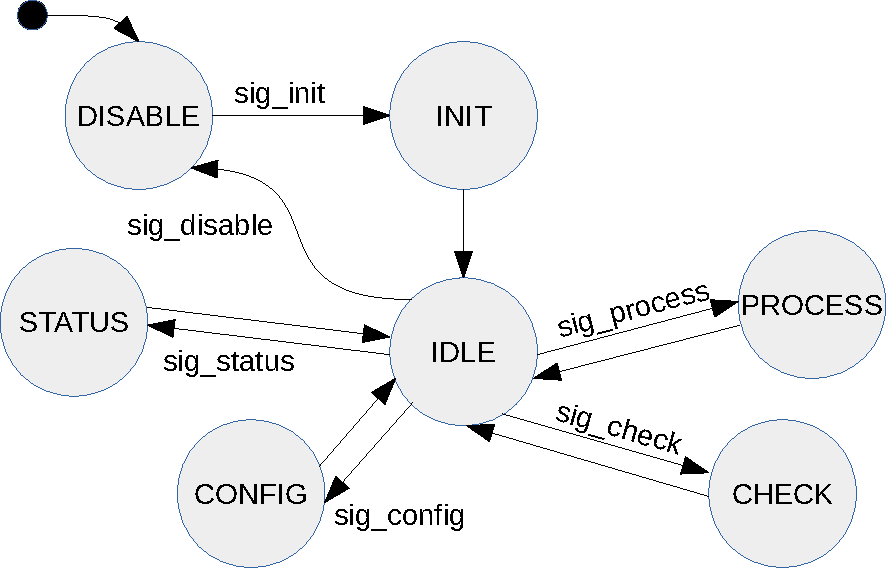
\includegraphics[width=\textwidth]{./Figures/MEF_HMI_2.pdf}
	\caption[MEF principal del módulo de HMI]{Máquina de estados finitos principal del módulo de interfaz máquina-hombre}
	\label{fig:mef_HMI}
\end{figure}

Se describen las principales acciones y actividades de cada estado en la tabla \ref{tab:estadosHMI}.  Asimismo, se indican las señales válidas que puede recibir la MEF junto con las transiciones que éstas provocan.


% Please add the following required packages to your document preamble:
% \usepackage{graphicx}
\begin{table}[htpb]
\centering
\caption[Descripción de los estados de la MEF principal del módulo HMI.]{Descripción de los estados de la MEF principal del módulo de interfaz máquina-hombre (HMI).  Se indican las señales que puede recibir junto con las acciones más relevantes de cada estado.}
\label{tab:estadosHMI}
\resizebox{\textwidth}{!}{%
\begin{tabular}{lll}
\toprule
\multicolumn{1}{c}{\textbf{Estado}} & \multicolumn{1}{c}{\textbf{Señal para cambio}} & \multicolumn{1}{c}{\textbf{Acciones y actividades}} \\ \midrule
DISABLE & Reset o sig\_disable & \begin{tabular}[c]{@{}l@{}}Desinicializar la UART.\\ Deshabilitar la interrupción de la UART. \\ Deshabilitar la transmisión de la UART\\ Cambiar el estado del módulo de READY a DISABLE.\end{tabular} \\
 &  &  \\
INIT & sig\_init & \begin{tabular}[c]{@{}l@{}}Inicializar la UART.\\ Habilitar la interrupción de la UART.\\ Habilitar la transmisión de la UART.\\ Cambiar el estado del módulo de DISABLE a READY.\end{tabular} \\
 &  &  \\
IDLE & transición incondicional & Cambiar estado del módulo de PROCESSING a READY. \\
 &  &  \\
CONFIG & sig\_config & Realizar cambios de configuración al módulo. \\
 &  &  \\
CHECK & sig\_check & Realizar autochequeo e informar al módulo de control \\
 &  &  \\
PROCESS & sig\_process & Procesar los comandos recibidos \\ 
 &  &  \\
STATUS & sig\_status & Enviar información de un módulo al usuario \\ \bottomrule
\end{tabular}%
}
\end{table}

\clearpage

\section{Módulo de control}
\label{sec:control}

% Chapter Template

\chapter{Ensayos y Resultados} % Main chapter title

\label{Chapter4} % Change X to a consecutive number; for referencing this chapter elsewhere, use \ref{ChapterX}

En este capítulo se describe la estrategia general de \textit{testing} del proyecto y se documentan los ensayos realizados en 3 niveles de abstracción: a nivel de función, a nivel de módulo y a nivel de sistema.

%----------------------------------------------------------------------------------------
%	SECTION 1
%----------------------------------------------------------------------------------------

\section{Test Master Plan}
\label{sec:masterPlan}

Para la elaboración de un \textit{Test Master Plan} se tomaron elementos del paradigma de desarrollo basado el pruebas o TDD (por sus siglas en inglés, \textit{Test Driven Development}) como fue mencionado en la subsección \ref{subsec:tdd}. 

Cabe destacar que en la planificación de las tareas del proyecto, primero se definieron los casos de prueba; luego se prepararon las herramientas de \textit{testing}; luego se implementaron los módulos y finalmente, se realizaron las pruebas. Esto puede observarse en el diagrama de \textit{Activity on Node} de la figura \ref{fig:AoN} en la sección \ref{sec:plan}.

En ese sentido, resultó necesario tener bien definidos los requisitos funcionales y sus criterios de aceptación.  Se debieron contemplar todos los casos posibles de uso, tanto exitosos como de error, con lo que se elaboró un documento \citep{TestMasterPlan} de casos de prueba por módulo  y de esta manera, se dio cumplimiento al requerimiento 1.2 indicado en la sección \ref{sec:requerimientos}.  

Se ensayó el código en 3 niveles distintos de abstracción: a nivel de función, de módulo y de sistema, según se documenta en las subsecciones \ref{subsec:unitarias}, \ref{subsec:pruebasFuncionales} y \ref{subsec:pruebasSistema}, respectivamente. 

Asimismo, las pruebas sobre los módulos fueron diseñadas para evaluar únicamente la lógica principal de funcionamiento.  En cada caso, se debió abstraer al módulo bajo ensayo de otras capas o servicios que pudieran interactuar con su lógica principal, para lo cual se simuló el resultado de dichas interacciones con \textit{mocks}. 


\subsection{Pruebas unitarias}
\label{subsec:unitarias}

[\textbf{hablar de ceedling}]

\begin{figure}[ht]
	\centering
	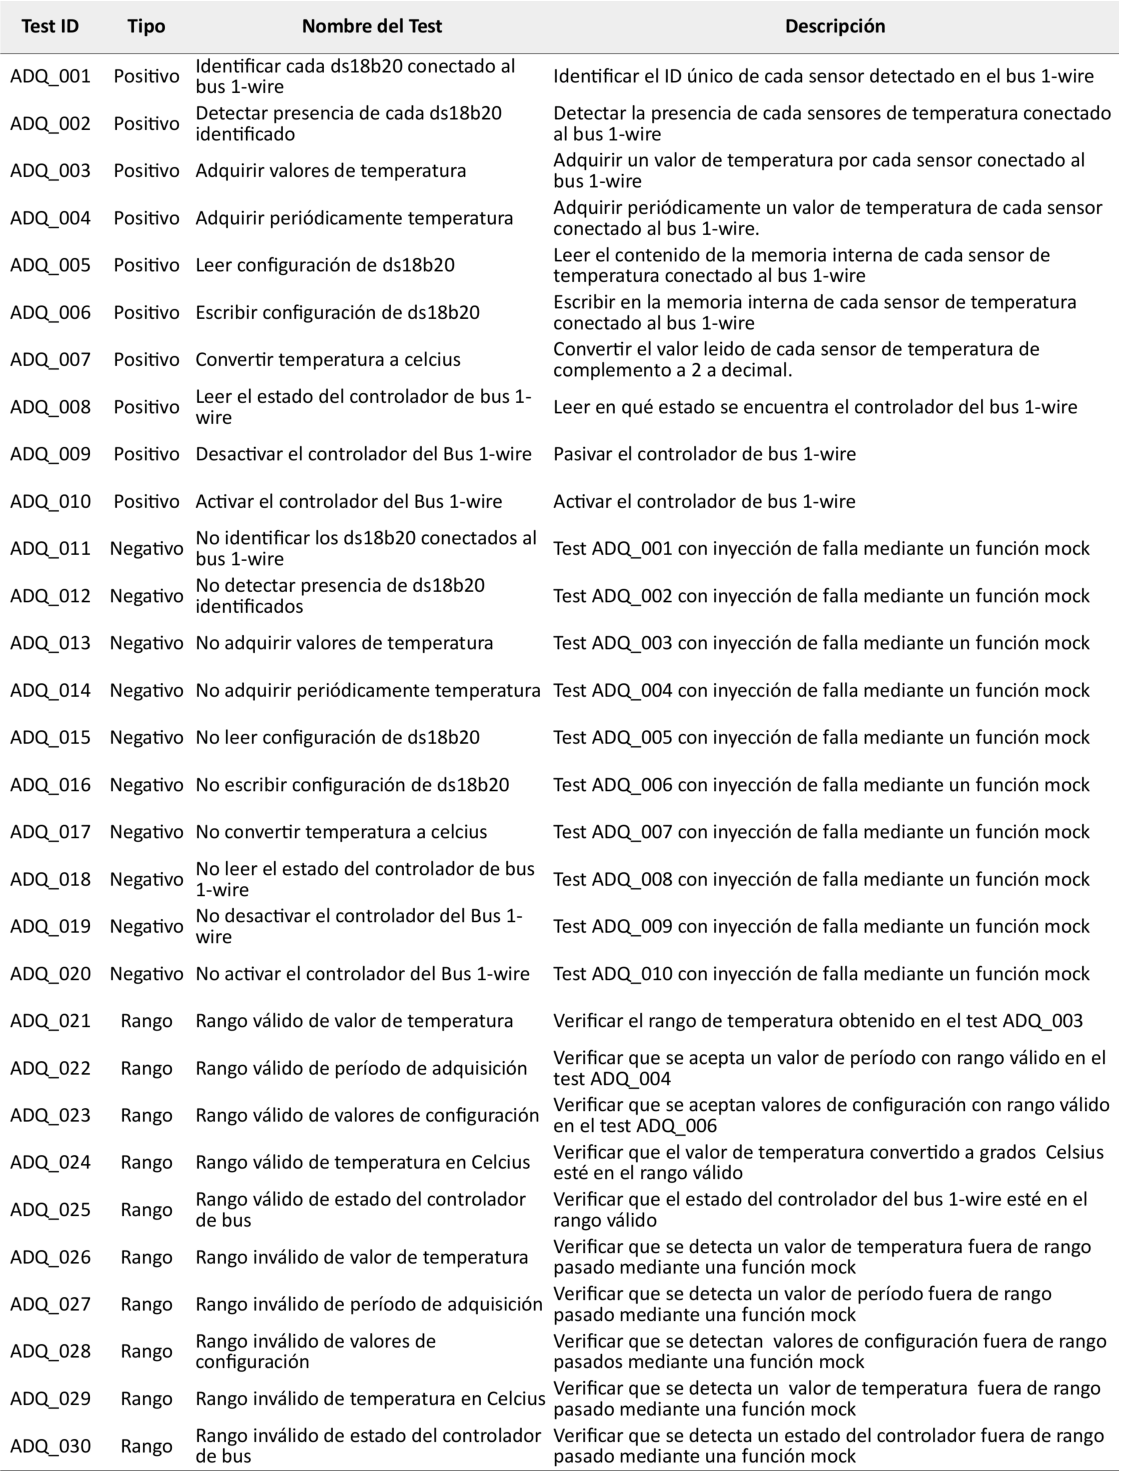
\includegraphics[width=\textwidth]{./Figures/TestADQ.pdf}
	\caption{algo}
	\label{fig:IPfC}
\end{figure}

\begin{figure}[ht]
	\centering
	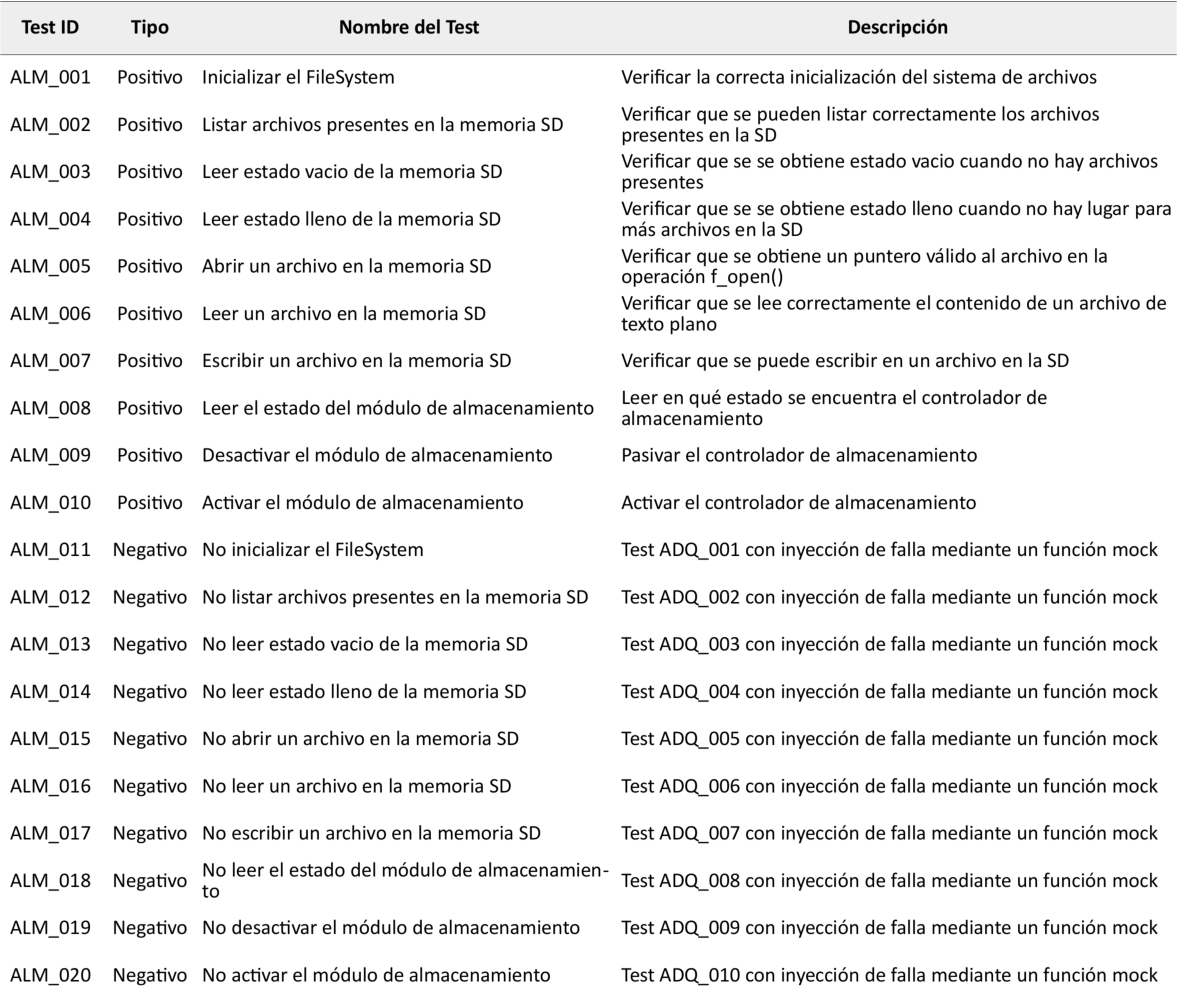
\includegraphics[width=\textwidth]{./Figures/TestSD.pdf}
	\caption{algo}
	\label{fig:IPfC}
\end{figure}

\subsection{Pruebas funcionales}
\label{subsec:pruebasFuncionales}


[\textbf{pruebas sobre las MEF de cada bloque}]

\subsection{Pruebas de sistema}
\label{subsec:pruebasSistema}

[\textbf{Pruebas}] 
% Chapter Template

\chapter{Conclusiones} % Main chapter title

\label{Chapter5} % Change X to a consecutive number; for referencing this chapter elsewhere, use \ref{ChapterX}

En este capítulo se destacan los principales aportes del trabajo realizado y se listan los logros obtenidos.  Asimismo, se documentan las técnicas que resultaron  útiles para la ejecución del proyecto.  Por otra parte, se deja constancia de las metas que no pudieron ser alcanzadas junto con las respectivas causas y se identifican las líneas de acción a futuro.
%----------------------------------------------------------------------------------------

%----------------------------------------------------------------------------------------
%	SECTION 1
%----------------------------------------------------------------------------------------

\section{Conclusiones generales }

%La idea de esta sección es resaltar cuáles son los principales aportes del trabajo realizado y cómo se podría continuar. Debe ser especialmente breve y concisa. Es buena idea usar un listado para enumerar los logros obtenidos.

En este trabajo se logró completar una primera iteración en el ciclo de diseño e implementación de un sistema embebido para el control de una estación de monitoreo de ruido ambiente submarino.  

Se pudo desarrollar un \textit{firmware} multicore modular que sienta las bases para una segunda iteración donde se diseñen e implementen tanto los componentes que quedaron fuera del alcance de esta etapa, así como también los que estaban contemplados pero no pudieron implementarse.

Los principales aportes de este trabajos son:

\begin{itemize}
	\item Adopción de una metodología de desarrollo basada en control de versiones sistemática y robusta.
	\item Desarrollo de una arquitectura modular multicore que permite el intercambio de funcionalidades entre procesadores de forma flexible.
	\item Implementación de mecanismos de comunicación y sincronización entre procesadores, basados en interrupciones cruzadas y colas de mensajes.
	\item Implementación de mecanismos de control y despacho de tareas y eventos.
	\item Desarrollo de cuatro módulos con funcionalidad de adquisición de datos, almacenamientos de datos, HMI y control del sistema, respectivamente. 
%	\item Implementación de mecanismos de control y autochequeo para aumentar la seguridad de operación del sistema.
	\item Documentación completa de ingeniería de detalle de los módulos desarrollados.
	\item Documentación completa de testing.
	\item Documentación completa de trazabilidad entre requerimientos, ingeniería de detalle y testing.
\end{itemize} 

\subsection{Técnicas útiles}
\label{subsec:tecnicas_utiles}

Resultaron particularmente útiles las técnicas de gestión de proyecto empleadas en la planificación de este trabajo.  Mediante el desglose del proyecto en tareas y la articulación de éstas en diagramas de \textit{Activity on Node} y \textit{Gantt}, se puedo definir una metodología de seguimiento y control que permitió detectar retrasos en el avance del proyecto. Se aplicaron medidas de mitigación \textit{ad-hoc} que consistieron en:

\begin{itemize}
	\item el incremento de la dedicación horaria destinada al proyecto,
	\item el empleo de funciones \textit{mock} o maquetadas para algunas características secundarias que pensaban implementarse.
	\item y en última instancia, la priorización del requerimiento implícito de fecha de finalización por sobre la cantidad de sensores operativos.
\end{itemize}  

%Este plan de acción neutralizó parcialmente los efectos negativos sobre el resultado del proyecto al costo de no cumplir .

Dentro de la gestión de riesgos no se contempló explícitamente la posibilidad de imprevistos como los que efectivamente se manifestaron.  Una análisis posterior de los hechos muestra que los retrasos responden principalmente a dos fuentes:

\begin{enumerate}
	\item un evento fortuito, único e irrepetible, en el ámbito laboral, que sobrecargó la dedicación horaria a tareas ajenas al proyecto durante gran parte de tiempo planificado para su realización e incluyó día de embarque.
	\item la incorporación de nuevas responsabilidades en el campo de la docencia.
\end{enumerate}

La primera fuente constituye un hecho aislado y, por su carácter de imprevisible, resulta razonable que haya quedado fuera del alcance de la gestión de riesgos.  

La segunda fuente implica un error de cálculo en la relación entre horas disponibles y la carga horaria de las tareas de docencia asumidas.  Esto último será tenido en cuenta como aprendizaje para futuros proyecto.

En términos generales, fue correcta la valoración de severidad y tasa de ocurrencia para todos los riesgos identificados; de los riesgos originalmente previstos:

\begin{enumerate}
	\item No contar a tiempo con el anemómetro.
	\item No contar con drivers para controlar el termómetro digital.
	\item No contar con el becario PIDDEF a tiempo para que pueda participar en el proyecto.
	\item Pérdida, robo o destrucción total o parcial de la placa CIAA-NXP y/o el anemómetro
	\item Cancelación del proyecto PIDDEF del Ministerio de Defensa asociado.
\end{enumerate}

\noindent sólo se manifestó íntegramente el riesgo número 3, que acertadamente fue valorado con una probabilidad de la ocurrencia alta. En este sentido, resultó adecuada la estrategia de planificar las tareas para ser llevadas a cabo sin la colaboración de un becario, por lo cual no se produjo ningún impacto negativo en el proyecto. 

Respecto al riesgo número 5, si bien el proyecto no fue cancelado, el hecho de contar con un subsidio trianual como el otorgado por el programa PIDDEF \citep{PIDDEF}, que haya coincidido con el cambio de gestión en la administración pública ocasionó retrasos y sobrecostos significativos que afortunadamente pudieron ser sobrellevados.

%En términos generales, fue correcta la valoración de severidad y tasa de ocurrencia para todos los riesgos identificados.

\subsection{Metas alcanzadas}
\label{subsec:metasalcanzadas}

Se recopila en la tabla \ref{tab:reqs_alcanzados} el estado de los requerimientos, indicando mediante un tilde y color verde los que fueron alcanzados satisfactoriamente.  Asimismo, se indica con una X y color rojo los requerimientos que no pudieron lograrse.

% Please add the following required packages to your document preamble:
% \usepackage{booktabs}
% \usepackage[table,xcdraw]{xcolor}
% If you use beamer only pass "xcolor=table" option, i.e. \documentclass[xcolor=table]{beamer}
\begin{table}[!htpb]
\centering
\caption{Requerimientos alcanzados.}
\label{tab:reqs_alcanzados}
\begin{tabular}{@{}lc@{}}
\toprule
%\rowcolor[HTML]{9B9B9B} 
\textbf{Requerimiento} & \textbf{Estado} \\ \midrule
\rowcolor[HTML]{EFEFEF} 
1. Requerimientos de documentación &  \\
 &  \\
 \rowcolor[HTML]{9AFF99} 
\begin{tabular}[c]{@{}l@{}}1.1 Se debe generar un Memoria Técnica con la documentación \\ de ingeniería detallada.\end{tabular} &  \checkmark \\
 &  \\
\rowcolor[HTML]{9AFF99} 
1.2 Se debe generar un documento de casos de prueba. &  \checkmark \\
 &  \\
\rowcolor[HTML]{EFEFEF} 
2. Requerimientos funcionales del sistema &  \\
 &  \\
\rowcolor[HTML]{9AFF99} 
\begin{tabular}[c]{@{}l@{}}2.1 El sistema debe adquirir datos de un array de sensores de \\ temperatura a intervalos regulares con un período de adquisición \\ seleccionable.\end{tabular} &  \checkmark \\
 &  \\
 \rowcolor[HTML]{FFCCC9} 
\begin{tabular}[c]{@{}l@{}}2.2 El sistema debe adquirir datos de un anemómetro a intervalos \\ regulares con un período de adquisición seleccionable.\end{tabular} &  X \\
 &  \\
\rowcolor[HTML]{9AFF99} 
\begin{tabular}[c]{@{}l@{}}2.3 El sistema debe almacenar los datos de temperatura y velocidad\\ de viento adquiridas junto con una marca de tiempo identificatoria \\ en un medio físico no volátil.\end{tabular} & \checkmark \\
 &  \\
\rowcolor[HTML]{9AFF99} 
\begin{tabular}[c]{@{}l@{}}2.4 El sistema debe poder operar con dos perfiles de consumo de \\ energía máximo desempeño y mínimo consumo de energía.\end{tabular} & \checkmark \\
 &  \\
 \rowcolor[HTML]{9AFF99} 
\begin{tabular}[c]{@{}l@{}}2.5 El sistema debe contar con una interfaz serie cableada que \\ permita realizar operaciones de configuración y mantenimiento.\end{tabular} & \checkmark \\
 &  \\
\rowcolor[HTML]{EFEFEF} 
3. Requerimientos de verificación &  \\
 &  \\
 \rowcolor[HTML]{9AFF99} 
\begin{tabular}[c]{@{}l@{}}3.1 Se debe generar una matriz de trazabilidad entre la Memoria\\ Técnica y los requerimientos.\end{tabular} & \checkmark \\
 &  \\
 \rowcolor[HTML]{9AFF99} 
\begin{tabular}[c]{@{}l@{}}3.2 Se debe generar una matriz de trazabilidad entre las pruebas \\ de integración y los requerimientos.\end{tabular} & \checkmark \\
 &  \\
\rowcolor[HTML]{EFEFEF} 
4. Requerimientos de validación &  \\
 &  \\
 \rowcolor[HTML]{9AFF99} 
\begin{tabular}[c]{@{}l@{}}4.1 Se debe generar una matriz de trazabilidad entre el documento\\ de casos de prueba y los requerimientos.\end{tabular} & \checkmark \\ \bottomrule
\end{tabular}
\end{table}

A los fines prácticos de terminar el trabajo en la fecha pactada, no fue posible implementar el control del anemómetro.  Esto no responde a una dificultad técnica sino a hechos imprevistos en la planificación que sobrecargaron la dedicación horaria a actividades ajenas al proyecto e imposibilitaron el cumplimiento del requisito asociado a este sensor como fuera mencionado en la subsección \ref{subsec:tecnicas_utiles}.

%----------------------------------------------------------------------------------------
%	SECTION 2
%----------------------------------------------------------------------------------------
\section{Próximos pasos}

Se indican en esta sección las líneas de acción más inmediatas para continuar la implementación del sistema e incorporar nuevas características a la estación de medición en desarrollo.  Asimismo se establece un orden de prioridad para las acciones identificadas, a saber:

\begin{enumerate}
  \item Implementar el control del anemómetro y completar los requerimientos previstos para esta etapa del proyecto.
  \item Reemplazar las funciones \textit{mock} que interactuan con la interfaz del sistema y así completar la implementación de todos los estados de las máquinas de estados finitos principales de cada módulo.
  \item Incorporar más opciones de configuración a cada módulo.  Para este fin, se contempla el pasaje por referencia de una estructura de configuración diferenciada para cada módulo que contenga los distintos parámetros configurables.  Asimismo, se debe reformular el diseño de la interfaz máquina-hombre para permitir la toma de dichos parámetros.
  \item Analizar la mejor forma de aprovechar las características asimétricas de los dos procesadores que posee la plataforma CIAA-NXP en cuanto a distribución de los módulos entre los procesadores.  La arquitectura desarrollada permite que el mismo código sea descargado a ambos procesadores, debiendo elegirse en un archivo de configuración qué módulo se ejecuta en qué procesador para que no ocurran colisiones a la hora de acceder a los recursos.  Esto permite explorar alternativas que aumenten la seguridad del sistema ante eventuales fallas de un procesador, existiendo redundancia de otro procesador que pueda retomar la ejecución de las tareas caídas.  Asimismo, resulta de interés evaluar el desempeño del sistema en cuanto a consumo eléctrico, disipación térmica y tiempo de cómputo, entre otras características, en diferentes configuraciones de reparto de módulos entre los procesadores.
  \item Incorporar al modelo de desarrollo un servidor de integración continua \citep{CI} para automatizar pruebas estáticas y dinámicas sobre el código.  
  \item Incorporar los subsistemas contemplados para futuras etapas en la figura \ref{fig:diagramaBloques} y que fueron considerados fuera del alcance en este proyecto, en forma de nuevos módulos de la estación, siguiendo el mismo patrón de diseño presentado en este trabajo.
  \item Diseñar y fabricar un pocho para la CIAA-NXP que permita conectar y desconectar en forma robusta las diferentes entradas y salidas del sistema de forma de poder operar la estación en condiciones de campo.
  \item Realizar pruebas de campo. 
\end{enumerate}


 

%----------------------------------------------------------------------------------------
%	CONTENIDO DE LA MEMORIA  - APÉNDICES
%----------------------------------------------------------------------------------------

\appendix % indicativo para indicarle a LaTeX los siguientes "capítulos" son apéndices

% Incluir los apéndices de la memoria como archivos separadas desde la carpeta Appendices
% Descomentar las líneas a medida que se escriben los apéndices

%% Appendix A

\chapter{Plantilla para casos de uso} % Main appendix title

\label{AppendixA} % Fo

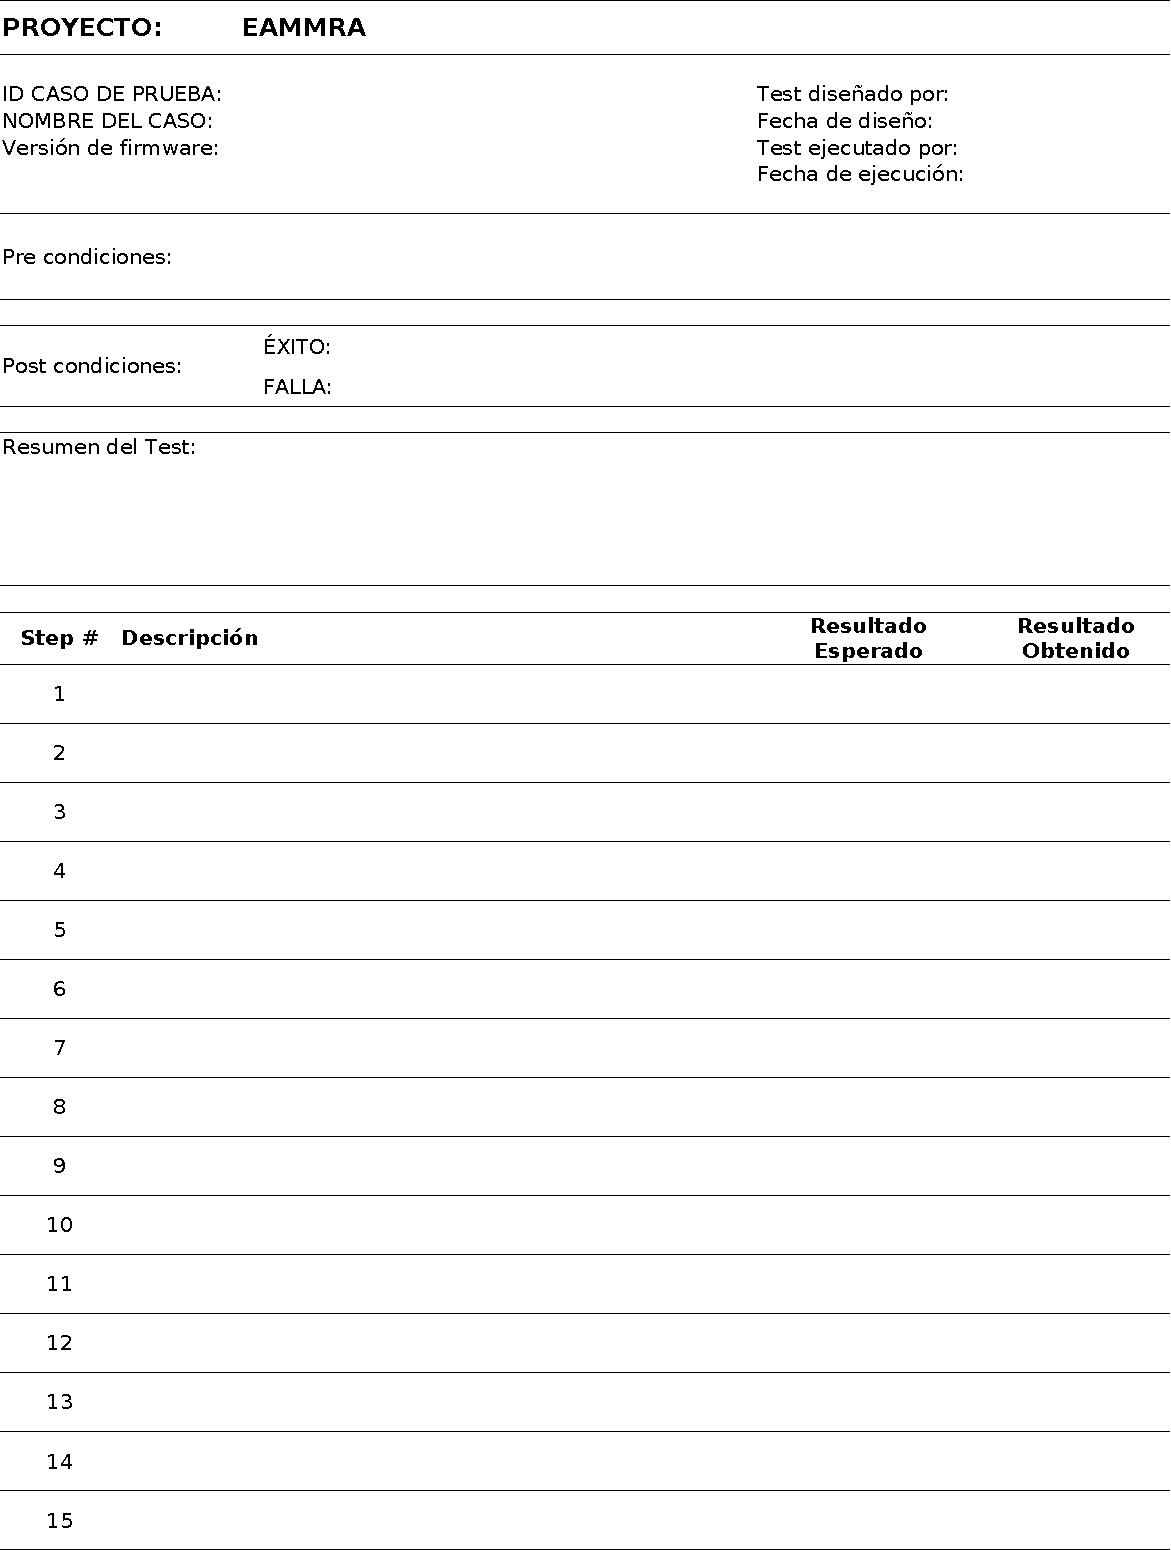
\includepdf[pages=-,scale=.8]{UseCaseTemplate.pdf}
%\include{Appendices/AppendixB}
%\include{Appendices/AppendixC}

%----------------------------------------------------------------------------------------
%	BIBLIOGRAPHY
%----------------------------------------------------------------------------------------

\Urlmuskip=0mu plus 1mu\relax
\raggedright
\printbibliography[heading=bibintoc]

%----------------------------------------------------------------------------------------

\end{document}  
